%  A simple AAU report template.
%  2013-03-06 v. 1.0.0
%  Copyright 2010-2013 by Jesper Kjær Nielsen <jkn@es.aau.dk>
%
%  This is free software: you can redistribute it and/or modify
%  it under the terms of the GNU General Public License as published by
%  the Free Software Foundation, either version 3 of the License, or
%  (at your option) any later version.
%
%  This is distributed in the hope that it will be useful,
%  but WITHOUT ANY WARRANTY; without even the implied warranty of
%  MERCHANTABILITY or FITNESS FOR A PARTICULAR PURPOSE.  See the
%  GNU General Public License for more details.
%
%  You can find the GNU General Public License at <http://www.gnu.org/licenses/>.
%
%  A simple AAU report template.
%  2013-03-06 v. 1.0.0
%  Copyright 2010-2013 by Jesper Kjær Nielsen <jkn@es.aau.dk>
%
%  This is free software: you can redistribute it and/or modify
%  it under the terms of the GNU General Public License as published by
%  the Free Software Foundation, either version 3 of the License, or
%  (at your option) any later version.
%
%  This is distributed in the hope that it will be useful,
%  but WITHOUT ANY WARRANTY; without even the implied warranty of
%  MERCHANTABILITY or FITNESS FOR A PARTICULAR PURPOSE.  See the
%  GNU General Public License for more details.
%
%  You can find the GNU General Public License at <http://www.gnu.org/licenses/>.
%
\documentclass[11pt,twoside,a4paper,openright]{report}
\setcounter{tocdepth}{1}
%%%%%%%%%%%%%%%%%%%%%%%%%%%%%%%%%%%%%%%%%%%%%%%%
% Language, Encoding and Fonts
% http://en.wikibooks.org/wiki/LaTeX/Internationalization
%%%%%%%%%%%%%%%%%%%%%%%%%%%%%%%%%%%%%%%%%%%%%%%%
% Select encoding of your inputs. Depends on
% your operating system and its default input
% encoding. Typically, you should use
%   Linux  : utf8 (most modern Linux distributions)
%            latin1 
%   Windows: ansinew
%            latin1 (works in most cases)
%   Mac    : applemac
% Notice that you can manually change the input
% encoding of your files by selecting "save as"
% an select the desired input encoding. 
\usepackage[utf8]{inputenc}
% Make latex understand and use the typographic
% rules of the language used in the document.
\usepackage[danish,english]{babel}
% Use the vector font Latin Modern which is going
% to be the default font in latex in the future.
\usepackage{lmodern}
% Choose the font encoding
\usepackage[T1]{fontenc}
%%%%%%%%%%%%%%%%%%%%%%%%%%%%%%%%%%%%%%%%%%%%%%%%
% Graphics and Tables
% http://en.wikibooks.org/wiki/LaTeX/Importing_Graphics
% http://en.wikibooks.org/wiki/LaTeX/Tables
% http://en.wikibooks.org/wiki/LaTeX/Colors
%%%%%%%%%%%%%%%%%%%%%%%%%%%%%%%%%%%%%%%%%%%%%%%%
% load a colour package
\usepackage{xcolor}
\definecolor{aaublue}{RGB}{33,26,82}% dark blue
% The standard graphics inclusion package
\usepackage{graphicx}
% Set up how figure and table captions are displayed
\usepackage{caption}
\captionsetup{%
  font=footnotesize,% set font size to footnotesize
  labelfont=bf % bold label (e.g., Figure 3.2) font
}
% Make the standard latex tables look so much better
\usepackage{array,booktabs}
% Enable the use of frames around, e.g., theorems
% The framed package is used in the example environment
\usepackage{framed}
\usepackage{tabularx}

%%%%%%%%%%%%%%%%%%%%%%%%%%%%%%%%%%%%%%%%%%%%%%%%
% Mathematics
% http://en.wikibooks.org/wiki/LaTeX/Mathematics
%%%%%%%%%%%%%%%%%%%%%%%%%%%%%%%%%%%%%%%%%%%%%%%%
% Defines new environments such as equation,
% align and split 
\usepackage{amsmath}
% Adds new math symbols
\usepackage{amssymb}
% Use theorems in your document
% The ntheorem package is also used for the example environment
% When using thmmarks, amsmath must be an option as well. Otherwise \eqref doesn't work anymore.
\usepackage[framed,amsmath,thmmarks]{ntheorem}

%%%%%%%%%%%%%%%%%%%%%%%%%%%%%%%%%%%%%%%%%%%%%%%%
% Page Layout
% http://en.wikibooks.org/wiki/LaTeX/Page_Layout
%%%%%%%%%%%%%%%%%%%%%%%%%%%%%%%%%%%%%%%%%%%%%%%%
% Change margins, papersize, etc of the document
\usepackage[
  left=28mm,% left margin on an odd page
  right=41mm,% right margin on an odd page
  ]{geometry}
% Modify how \chapter, \section, etc. look
% The titlesec package is very configureable
\usepackage{titlesec}
\titleformat*{\section}{\normalfont\Large\bfseries\color{aaublue}}
\titleformat*{\subsection}{\normalfont\large\bfseries\color{aaublue}}
\titleformat*{\subsubsection}{\normalfont\normalsize\bfseries\color{aaublue}}
%\titleformat*{\paragraph}{\normalfont\normalsize\bfseries\color{aaublue}}
%\titleformat*{\subparagraph}{\normalfont\normalsize\bfseries\color{aaublue}}

% Change the headers and footers
\usepackage{fancyhdr}
\pagestyle{fancy}
\fancyhf{} %delete everything
\renewcommand{\headrulewidth}{0pt} %remove the horizontal line in the header
\fancyhead[RE]{\color{aaublue}\small\nouppercase\leftmark} %even page - chapter title
\fancyhead[LO]{\color{aaublue}\small\nouppercase\rightmark} %uneven page - section title
\fancyhead[LE,RO]{\thepage} %page number on all pages
% Do not stretch the content of a page. Instead,
% insert white space at the bottom of the page
\raggedbottom
% Enable arithmetics with length. Useful when
% typesetting the layout.
\usepackage{calc}
\usepackage{graphicx}
\graphicspath{ {./figures/}{./figures/prototypes/} }
\usepackage{subcaption}
%%%%%%%%%%%%%%%%%%%%%%%%%%%%%%%%%%%%%%%%%%%%%%%%
% Bibliography
% http://en.wikibooks.org/wiki/LaTeX/Bibliography_Management
%%%%%%%%%%%%%%%%%%%%%%%%%%%%%%%%%%%%%%%%%%%%%%%%
% Add the \citep{key} command which display a
% reference as [author, year]
\usepackage[backend=bibtex,
  bibencoding=utf8
  ]{biblatex}
\addbibresource{bib/mybib}
%\usepackage[square]{natbib}
% Appearance of the bibliography
%\bibliographystyle{apalike}
\usepackage{csquotes}
\renewcommand{\mkbegdispquote}[2]{\itshape}
%%%%%%%%%%%%%%%%%%%%%%%%%%%%%%%%%%%%%%%%%%%%%%%%
% Misc
%%%%%%%%%%%%%%%%%%%%%%%%%%%%%%%%%%%%%%%%%%%%%%%%
% Add bibliography and index to the table of
% contents
\usepackage[nottoc]{tocbibind}
% Add the command \pageref{LastPage} which refers to the
% page number of the last page
\usepackage[
%  disable, %turn off todonotes
  colorinlistoftodos, %enable a coloured square in the list of todos
  textwidth=\marginparwidth, %set the width of the todonotes
  textsize=scriptsize, %size of the text in the todonotes
  ]{todonotes}
% added by KK (ShareLaTeX team)
\usepackage{lastpage}

%%%%%%%%%%%%%%%%%%%%%%%%%%%%%%%%%%%%%%%%%%%%%%%%
% Hyperlinks
% http://en.wikibooks.org/wiki/LaTeX/Hyperlinks
%%%%%%%%%%%%%%%%%%%%%%%%%%%%%%%%%%%%%%%%%%%%%%%%
% Enable hyperlinks and insert info into the pdf
% file. Hypperref should be loaded as one of the 
% last packages
\usepackage{hyperref}
\hypersetup{%
%	pdfpagelabels=true,%
	plainpages=false,%
	pdfauthor={Author(s)},%
	pdftitle={Title},%
	pdfsubject={Subject},%
	bookmarksnumbered=true,%
	colorlinks,%
	citecolor=aaublue,%
	filecolor=aaublue,%
	linkcolor=aaublue,% you should probably change this to black before printing
	urlcolor=aaublue,%
	pdfstartview=FitH%
}
\usepackage{wrapfig}


% LST Listings
\definecolor{bluekeywords}{rgb}{0,0,1}
\definecolor{greencomments}{rgb}{0,0.5,0}
\definecolor{redstrings}{rgb}{0.64,0.08,0.08}
\definecolor{xmlcomments}{rgb}{0.5,0.5,0.5}
\definecolor{types}{rgb}{0.17,0.57,0.68}

\definecolor{ForrestGreen}{RGB}{0,100,0}
\usepackage{listings}
\lstset{language=C,
literate=%
{æ}{{\ae}}1
{å}{{\aa}}1
{ø}{{\o}}1
{Æ}{{\AE}}1
{Å}{{\AA}}1
{Ø}{{\O}}1,
captionpos=t,
frame=lines,
numbers=left,
stepnumber=1,
showspaces=false,
showtabs=false,
breaklines=true,
showstringspaces=false,
breakatwhitespace=true,
escapeinside={(*@}{@*)},
commentstyle=\color{greencomments},
morecomment=[l]{\# },
keywordstyle=\color{bluekeywords},
emph={class, true, false, public, private, override, Time, Input, Random, KeyCode, Debug, using, StreamReader, Path, Environment, new, Length, OrderBy, ToArray, Count, Range, ExecuteNonQuery, Parameters, SqlCommand, AddWithValue},          
emphstyle=\ttfamily\color{ForrestGreen}, 
morekeywords={partial,var,value,class},
stringstyle=\color{redstrings},
basicstyle=\ttfamily\small,
classoffset=1, % starting new class
morekeywords={bool, boolean, float, double, Vector1, Vector2, Vector3, string, char, var, foreach, try, finally, Math, text, number, catch},
otherkeywords={bool, boolean, float, double, Vector1, Vector2, Vector3, string, char, var, foreach, try, finally, Math, text, number, catch},
keywordstyle=\color{bluekeywords},
classoffset=0,
}

\usepackage[normalem]{ulem}
\useunder{\uline}{\ul}{}

\usepackage{booktabs}
\usepackage{lscape}

% Command to rotate a text -90 degrees.
\newcommand*\rot{\rotatebox{-90}}

\usepackage{float}

\usepackage{pdfpages}

\usepackage{tikz}
\usetikzlibrary{calc,trees,positioning,arrows,chains,shapes.geometric,%
    decorations.pathreplacing,decorations.pathmorphing,shapes,%
    matrix,shapes.symbols}
    
\tikzset{
>=stealth',
  punktchain/.style={
    rectangle, 
    rounded corners, 
    % fill=black!10,
    draw=black, very thick,
    text width=10em, 
    minimum height=3em, 
    text centered, 
    on chain},
  line/.style={draw, thick, <-},
  element/.style={
    tape,
    top color=white,
    bottom color=blue!50!black!60!,
    minimum width=8em,
    draw=blue!40!black!90, very thick,
    text width=10em, 
    minimum height=3.5em, 
    text centered, 
    on chain},
  every join/.style={->, thick,shorten >=1pt},
  decoration={brace},
  tuborg/.style={decorate},
  tubnode/.style={midway, right=2pt},
}

\usepackage{mathtools}

\usepackage{graphicx}
\graphicspath{ {./figures/}{./figures/prototype-comp/} }
\usepackage{subcaption}

\usepackage{rotating}

\usepackage{amssymb}

\usepackage{tabularx}% package inclusion and set up of the document
% see, e.g., http://en.wikibooks.org/wiki/LaTeX/Formatting#Hyphenation
% for more information on word hyphenation
\hyphenation{ex-am-ple hy-phen-a-tion short}
\hyphenation{long la-tex}
% 
%  A simple AAU report template.
%  2013-03-06 v. 1.0.0
%  Copyright 2010-2013 by Jesper Kjær Nielsen <jkn@es.aau.dk>
%
%  This is free software: you can redistribute it and/or modify
%  it under the terms of the GNU General Public License as published by
%  the Free Software Foundation, either version 3 of the License, or
%  (at your option) any later version.
%
%  This is distributed in the hope that it will be useful,
%  but WITHOUT ANY WARRANTY; without even the implied warranty of
%  MERCHANTABILITY or FITNESS FOR A PARTICULAR PURPOSE.  See the
%  GNU General Public License for more details.
%
%  You can find the GNU General Public License at <http://www.gnu.org/licenses/>.
%
%
%
% see, e.g., http://en.wikibooks.org/wiki/LaTeX/Customizing_LaTeX#New_commands
% for more information on how to create macros

%%%%%%%%%%%%%%%%%%%%%%%%%%%%%%%%%%%%%%%%%%%%%%%%
% Macros for the titlepage
%%%%%%%%%%%%%%%%%%%%%%%%%%%%%%%%%%%%%%%%%%%%%%%%
%Creates the aau titlepage
\newcommand{\aautitlepage}[3]{%
  {
    %set up various length
    \ifx\titlepageleftcolumnwidth\undefined
      \newlength{\titlepageleftcolumnwidth}
      \newlength{\titlepagerightcolumnwidth}
    \fi
    \setlength{\titlepageleftcolumnwidth}{0.5\textwidth-\tabcolsep}
    \setlength{\titlepagerightcolumnwidth}{\textwidth-2\tabcolsep-\titlepageleftcolumnwidth}
    %create title page
    \thispagestyle{empty}
    \noindent%
    \begin{tabular}{@{}ll@{}}
      \parbox{\titlepageleftcolumnwidth}{
        \iflanguage{danish}{%
          
\includegraphics[width=\titlepageleftcolumnwidth]{figures/aau_logo_da}
        }{%
          
\includegraphics[width=\titlepageleftcolumnwidth]{figures/aau_logo_en}
        }
      } &
      \parbox{\titlepagerightcolumnwidth}{\raggedleft\sf\small
        #2
      }\bigskip\\
       #1 &
      \parbox[t]{\titlepagerightcolumnwidth}{%
      \textbf{Abstract:}\bigskip\par
        \fbox{\parbox{\titlepagerightcolumnwidth-2\fboxsep-2\fboxrule}{%
          #3
        }}
      }\\
    \end{tabular}
    \vfill
    \iflanguage{danish}{%
      \noindent{\footnotesize\emph{Rapportens indhold er frit tilgængeligt, men offentliggørelse (med kildeangivelse) må kun ske efter aftale med forfatterne.}}
    }{%
      \noindent{\footnotesize\emph{The content of this report is freely available, but publication (with reference) may only be pursued due to agreement with the author.}}
    }
    \clearpage
  }
}

%Create english project info
\newcommand{\englishprojectinfo}[8]{%
  \parbox[t]{\titlepageleftcolumnwidth}{
    \textbf{Title:}\\ #1\bigskip\par
    \textbf{Theme:}\\ #2\bigskip\par
    \textbf{Project Period:}\\ #3\bigskip\par
    \textbf{Project Group:}\\ #4\bigskip\par
    \textbf{Participant(s):}\\ #5\bigskip\par
    \textbf{Supervisor(s):}\\ #6\bigskip\par
    \textbf{Copies:} #7\bigskip\par
    \textbf{Page Numbers:} \pageref{LastPage}\bigskip\par
    \textbf{Date of Completion:}\\ #8
  }
}

%Create danish project info
\newcommand{\danishprojectinfo}[8]{%
  \parbox[t]{\titlepageleftcolumnwidth}{
    \textbf{Titel:}\\ #1\bigskip\par
    \textbf{Tema:}\\ #2\bigskip\par
    \textbf{Projektperiode:}\\ #3\bigskip\par
    \textbf{Projektgruppe:}\\ #4\bigskip\par
    \textbf{Deltager(e):}\\ #5\bigskip\par
    \textbf{Vejleder(e):}\\ #6\bigskip\par
    \textbf{Oplagstal:} #7\bigskip\par
    \textbf{Sidetal:} \pageref{LastPage}\bigskip\par
    \textbf{Afleveringsdato:}\\ #8
  }
}

%%%%%%%%%%%%%%%%%%%%%%%%%%%%%%%%%%%%%%%%%%%%%%%%
% An example environment
%%%%%%%%%%%%%%%%%%%%%%%%%%%%%%%%%%%%%%%%%%%%%%%%
\theoremheaderfont{\normalfont\bfseries}
\theorembodyfont{\normalfont}
\theoremstyle{break}
\def\theoremframecommand{{\color{aaublue!50}\vrule width 5pt \hspace{5pt}}}
\newshadedtheorem{exa}{Example}[chapter]
\newenvironment{example}[1]{%
		\begin{exa}[#1]
}{%
		\end{exa}
}
% my new macros
%\titleformat{\chapter}[hang]{\normalfont\huge\bfseries}{\thechapter}{1em}{}
%\titleformat{\section}
%{\normalfont\LARGE\bfseries}{\thesection}{1em}{}
%\titleformat{\subsection}
%{\normalfont\Large\bfseries}{\thesubsection}{1em}{}
%\titleformat{\subsubsection}
%{\normalfont\large\bfseries}{\thesubsubsection}{1em}{}
%\titlespacing\chapter{0pt}{-20pt}{20pt}
%\titlespacing\section{0pt}{12pt plus 4pt minus 2pt}{-2pt plus 2pt minus 2pt}
%\titlespacing\subsection{0pt}{12pt plus 4pt minus 2pt}{-2pt plus 2pt minus 2pt}
%\titlespacing\subsubsection{0pt}{12pt plus 4pt minus 2pt}{-2pt plus 2pt minus 2pt}

\begin{document}
%frontmatter
\pagestyle{empty} %disable headers and footers
\pagenumbering{roman} %use roman page numbering in the frontmatter
%  A simple AAU report template.
%  2013-03-06 v. 1.0.0
%  Copyright 2010-2013 by Jesper Kjær Nielsen <jkn@es.aau.dk>
%
%  This is free software: you can redistribute it and/or modify
%  it under the terms of the GNU General Public License as published by
%  the Free Software Foundation, either version 3 of the License, or
%  (at your option) any later version.
%
%  This is distributed in the hope that it will be useful,
%  but WITHOUT ANY WARRANTY; without even the implied warranty of
%  MERCHANTABILITY or FITNESS FOR A PARTICULAR PURPOSE.  See the
%  GNU General Public License for more details.
%
%  You can find the GNU General Public License at <http://www.gnu.org/licenses/>.
%
\pdfbookmark[0]{Front page}{label:frontpage}%
\begin{titlepage}
  \addtolength{\hoffset}{0.5\evensidemargin-0.5\oddsidemargin} %set equal margins on the frontpage - remove this line if you want default margins
  \noindent%
  \begin{tabular}{@{}p{\textwidth}@{}}
    \toprule[2pt]
    \midrule
    \vspace{0.2cm}
    \begin{center}
    \Huge{\textbf{
      Title of the project
    }}
    \end{center}
    \begin{center}
      \Large{
        Subtitle
      }
    \end{center}
    \vspace{0.2cm}\\
    \midrule
    \toprule[2pt]
  \end{tabular}
  \vspace{4 cm}
  \begin{center}
    {\large
      Project Report%Insert document type (e.g., Project Report)
    }\\
    \vspace{0.2cm}
    {\Large
      Group: SW805F20%Insert your group name or real names here
    }
  \end{center}
  \vfill
  \begin{center}
  Aalborg University\\
  Department of Computer Science\\
  Selma Lagerlöfs Vej 300\\
  9220 Aalborg East, DK
  \end{center}
\end{titlepage}
\clearpage

\thispagestyle{empty}
{\small
\strut\vfill % push the content to the bottom of the page
\noindent Copyright \copyright{} Aalborg University 2019\par
\vspace{0.2cm}
\noindent Photographic, mechanic or any other form of duplication of this paper is not allowed according to Danish copyright law and without permission by the authors.
}
\clearpage


\pdfbookmark[0]{English title page}{label:titlepage_en}
\aautitlepage{%
  \englishprojectinfo{
    Innovation and Mobility for a Location Based Virtual Reality Game%title
  }{%
     Mobility %theme
  }{%
    Spring Semester 2020 %project period
  }{%
    SW805F20 % project group
  }{%
    %list of group members
    Andreas Stenshøj\\
    Daniel Moesgaard Andersen\\
    Frederik Valdemar Schrøder\\
    Jens Petur Tróndarson\\
    Rasmus Bundgaard Eduardsen\\
    Mathias Møller Lybech
  }{%
    %list of supervisors
    Brian Nielsen\\
  }{%
    1 % number of printed copies
  }{%
    May 28th, 2020 % date of completion
  }%
}{%department and address
  \textbf{Department of Computer Science}\\
  Aalborg University\\
  Selma Lagerlöfs Vej 300\\
  9220 Aalborg East, DK\\
  \href{www.cs.aau.dk}{www.cs.aau.dk}
}{% the abstract
  abstractus
}

\cleardoublepage
\pdfbookmark[0]{Contents}{label:contents}
\pagestyle{fancy} %enable headers and footers again
\tableofcontents
\chapter{Resources}\label{resources}
The code for the project can be found in the following GitHub repositories:

\section*{Host software}
\hyperlink{https://github.com/SW805F20/pozyx-location-tracker}{https://github.com/SW805F20/pozyx-location-tracker}

\section*{Client game}
\hyperlink{https://github.com/SW805F20/Unity}{https://github.com/SW805F20/Unity}

\chapter*{Terms and abbreviations}
Terms and abbreviations used in the report:
\begin{align*}
    %define these two
    \textbf{Pozyx}    & : \text{The hardware used for positioning.} \\
    \textbf{AR}       & : \text{Augmented reality.}                 \\
    \textbf{UWB}      & : \text{Ultra-wide bandwidth.}              \\
    \textbf{TWR}      & : \text{Two-way-ranging.}                   \\
    \textbf{MVP}      & : \text{Minimum viable product.}            \\
    \textbf{OSI}      & : \text{Open systems interconnection.}      \\
    \textbf{GDOP}     & : \text{Geometric Dilution of Precision.}   \\
    \textbf{TCP}      & : \text{Transmission Control Protocol.}     \\
    \textbf{UDP}      & : \text{User Datagram Protocol.}            \\
    \textbf{Zeroconf} & : \text{Zero Configuration Networking.}     \\
    \textbf{DoD}      & : \text{Definition of done.}                \\
\end{align*}
\cleardoublepage
%mainmatter
\pagenumbering{arabic} %use arabic page numbering in the mainmatter
\chapter{Introduction}
\section{Project idea}\label{sec:projectidea}
The idea for this project is to create a location-based competitive game using augmented reality (AR).
Two teams will compete against each other to score the most goals using a ball. 
Each player will be equipped with a smartphone-based virtual reality headset, and these will display the playing field from a top-down 2D view. 
To achieve this, each player's position needs to be tracked as well as where the ball is located on the field.
In the top-down view, each player needs to see the positions of the other players and the ball.
They also need to see their position on the playing field and where the goals are.
The players should be able to set a number of goals they need to score to win before beginning the game. 
\begin{figure}[H]
    \centering
    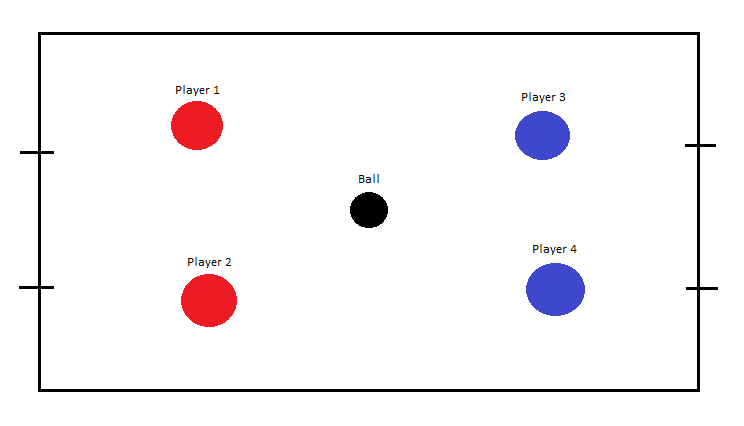
\includegraphics[width=0.6\linewidth]{Spil.PNG}
    \caption{An illustration of the playing field}
    \label{fig:game_illustration}
\end{figure}
\noindent
In \autoref{fig:game_illustration}, an illustration of the playing field for the game is shown.
There are goals at each end of the field, and the teams score goals by getting the ball between the goalposts.
An alternative version of the game is suggested where, instead of goals at each end of the field, there would be virtual goal zones seen in the game which the teams need to bring the ball into.
These zones could even change locations as the game progressed.

\subsection{Technical requirements for the project}
Various hardware will be required to realize the vision of the game.
First of all, each player must have a headset to hold their smartphone such that they can view a virtualized version of the playing field while playing.
In order for the data to be synchronized between the players, they will also need to be equipped with a positioning device, which can transmit their location to the other players.
This transfer of information will require a networking solution so that the virtualized playing field is synchronized between the players.

\subsection{Problems to consider}
The initial project idea proposes some problems that will need to be solved for the game to work.
We will need to consider which technologies to use for the development of the visual aspect of the game which should show a top-down view for each player. 
As we do not have experience creating VR-based games, it would be preferable if it is not necessary to have to build it from scratch.\\
Additionally, hardware that can track the positions of players and the ball is needed.
This must be accurate and update quickly such that the players do not run into each other, otherwise the game will not work.
Another problem to consider is how the ball should be displayed in a 2D view.
For the players to be able to find the ball on the field, it either has to be quite large to make it easier to find from the top-down view, or the game will need some metric to display how far the ball is from the ground.
The game will also need to track when the ball has crossed the goal line and then give feedback to the players.
Another problem to solve is how to keep the positional data synchronized across all the players' devices, as it will be difficult to play the game without accurate data.

\chapter{Sprint 1}
\section{Unity introduction}\label{sec:unity-intro}
As defined in \autoref{sec:projectidea}, this project aims to create a location-based augmented reality game.
This means the project has to have a game component - an application to display the objectives of the game, the play area, and the players.
To create this, a game engine can be used, such as \texttt{Unity}. \\
A game engine is a piece of software that provides creators with the necessary set of features to develop games quickly and efficiently \cite{gameengine}.
This means that a game engine is a collection of reusable components, abstracted away from the game developer.
This can include tools to help with, for example, graphics, physics, networking or audio.
These tools would expose certain functionality to a developer to make use of, and hide the specific implementation details for that functionality, ensuring the developer can focus on more pressing issues.
Unity supports the C\# language for development \cite{unitylanguage}.
\\\\
The Unity game engine supports development for different game platforms.
Of particular interest to this project is the support for both \texttt{Android} and \texttt{iOS} devices, as well as \texttt{Google Cardboard} \cite{unityplatforms}.\\
Unity was chosen for the development of the game aspect of this project since this facilitates that a greater amount of time can be spent on the other aspects of the project rather than the low-level details of game development, and it allows for easier inclusion of multiple platforms.

\chapter{Sprint 2}
The second sprint lasted 3 weeks from March 4th to March 25th.
\section{Sprint goal and introduction}\label{sec:sprint2-goals}
The goal for this sprint is to explore the networking side of the project and implement initial versions of the UDP client and server based on what was learned in \autoref{sec:sprint1-networking}.
Additionally, the first version of the game should be created, which should allow players to see the game through VR goggles and show the players moving based on the positions of the tags.

\section{Deployment Diagram}\label{sec:sprint2-deploymentdia}
\autoref{sec:sprint1-architecture} introduced the different components of the system in \autoref{fig:architecture}.
In order to further elaborate on the different components, a deployment diagram is constructed.
\begin{figure}[H]
    \centering
    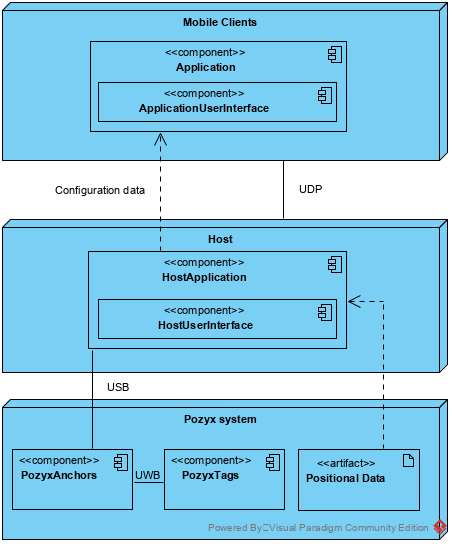
\includegraphics[width=0.6\linewidth]{deploymentdiagram1.png}
    \caption{A deployment diagram for the system.}
    \label{fig:sprint2-deployment}
\end{figure}
\noindent
A deployed system will contain three nodes:
\begin{itemize}
    \item Pozyx system
    \item Host
    \item Mobile Clients
\end{itemize}
Nodes are represented by cubes, and are entities executing components.
The Pozyx system node contains two components.
These are the anchors and the tags needed to generate positioning data with the Pozyx hardware.
The system contains multiples of each.
These Pozyx components generate artifacts in terms of positional data for the location of the players and the ball.
Anchors and tags are associated through a UWB connection in order to generate the artifacts.
The host node is dependent on the positional data artifact, the component receives the positional data and transforms it for communication.
Positional data is transferred from the Pozyx system to the host through a USB association.
The host application component contains a user interface component, which is the interface that the person using the host component will interact with, in the form of a terminal application for the early version of the system.
The host node is associated with the clients through a UDP connection in order to communicate both the positional data and configuration data to perform game setup.
As such, the mobile client application component is dependent on the host application component, since it needs the configuration data.
The mobile clients also contain user interface components, which is how the users interact with that part of the system.
This user interface is the virtual playing field generated in Unity that the users view in the headset.

\section{Accessing games on the network}
Different methods of transmission were discussed in \autoref{sec:sprint1-udptransmission}, and multicasting was selected as the optimal solution for this project.
In order to make proper use of this in an eventual deployment of the game, it would not make sense for the users to input the IP address to which they want to connect.
As such, a way to access hosted games without this needs to be implemented.
In order to support multiple games being played at the same time, the system also needs to properly make use of multicast groups based on the game being joined.
Clients should only receive data from one specific host in their specific multicast group.
\\\\
To do this, the game must include some form of LAN discoverability.
One way of achieving this is to have clients searching for a game broadcast a message to available hosts via the LAN.
The hosts then reply if they are available along with data for a multicast group, and the client can then join that group.
Another method could be to make use of Internet Group Management Protocol(IGMP), which is a communications protocol used on IPv4 networks to establish multicast groups.
The IP address 224.0.0.1 is a notable IPv4 address reserved for IP multicasting, which is the multicast group address for all hosts on the sane network \cite{ipv4multicastaddresses}.
All hosts should join that group on start-up, and clients could then message the group that they are looking for an available game.
\\\\
Another way would be to have the host continually broadcast messages that it is available for players.
This would, however, lead to the host needing to repeatedly send messages for as long as it is not filled with players or has not started.
This would likely be a less elegant solution than having players searching for hosts message a couple of times.
\\\\
Having the players send a message to the multicast group address for all hosts is the preferable solution, as it will avoid unnecessary overhead caused by broadcast messages being sent to unrelated machines on the network.
In order to select a game to join as a client, the game would need a game selection screen.
\autoref{fig:prototype:menu} and \autoref{fig:prototype:menuconnected} show the initial prototypes for joining a host-based on their IP and waiting for the game to begin.
If a lobby were to be implemented, \autoref{fig:prototype:menu} would need to be updated, and there would need to be an extra step before \autoref{fig:prototype:menuconnected} could be shown.
\autoref{fig:sprint2:prototype:menu} and \autoref{fig:sprint2:prototype:lobby} show new prototypes for this purpose.
Choosing a lobby on \autoref{fig:sprint2:prototype:lobby} would lead to \autoref{fig:prototype:menuconnected}.
\begin{figure}[H]
    \centering
    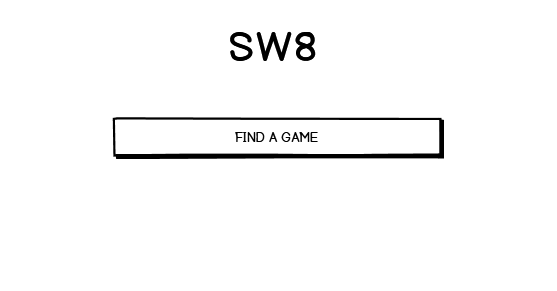
\includegraphics[width=0.6\linewidth]{prototypes/sprint2-menu.png}
    \caption{Prototype of game menu when players can choose a game to join. They need to either search for games or host one.}
    \label{fig:sprint2:prototype:menu}
\end{figure}

\begin{figure}[H]
    \centering
    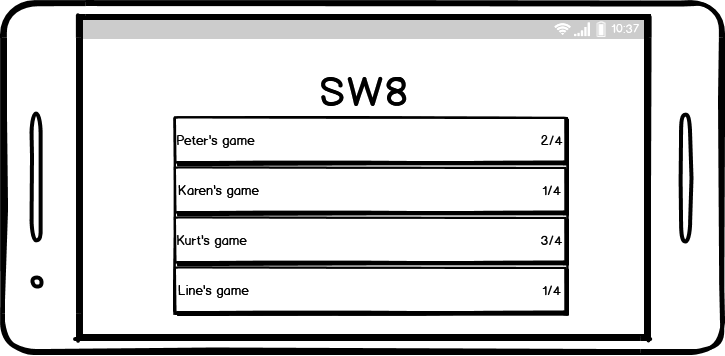
\includegraphics[width=0.6\linewidth]{prototypes/sprint2-lobby.png}
    \caption{Prototype of a lobby menu. Available games are shown as well as the number of players. Players can choose one to join.}
    \label{fig:sprint2:prototype:lobby}
\end{figure}

\section{UDP implementation}
In this section, we will delve into the implementation details of the UDP client and host.
As described in \autoref{sec:sprint2-deploymentdia}, the system will consist of a host computer which receives positional data from Pozyx and transmits it to the players using IP multicasting.

\subsubsection{Host}
The main functionality of the host is to transmit positional data from the Pozyx tags to the clients via multicasting.
The first setup step of this is to connect the host to an IP address on the network dedicated to multicasting, as described in \autoref{sec:accessonnetwork}.
For the time being, this is hardcoded to be \texttt{224.3.29.71:10000}.

After this initial setup, the host will continuously run through a loop where it updates the ball position, player positions and increments the timestamp.

Each update consists of three steps: Getting the positional data from Pozyx, transforming it to fit the format described in \autoref{subsec:dataform} and transmitting the data to the clients, as seen on \autoref{lst:updateballposition}.

\begin{lstlisting}[caption={Updating ball position},language=Python,label={lst:updateballposition}]
def update_ball_position(self):
    """Broadcasts the updated ball position"""
    ball_tag = self.setup.ball_tag
    position = self.multi_tag_positioning.get_position(ball_tag)
    message = self.formatter.format_player_position(self.time_stamp, 0, position.x, position.y)
    self.multicast_sender.send(message)
\end{lstlisting}


\subsubsection{Client}
Like the host, the client joins the multicast group on the specified IP.
While the host continuously sends positional data, the client's job is to receive and react to the data that is being sent to the multicast.
This is done by creating an asynchronous callback, which ensures that the data receiver is called whenever data is being transmitted, which is seen on the first three lines of \autoref{lst:receivedata}.
Once the \texttt{Receive} function is called, it saves the received bytes to an array and starts listening for new data before it starts working with the data.
This was done to ensure that new messages would not be blocked if it takes too long to handle the data.

In the current version, the receiver will simply log the data to the Unity console, but in future versions, it will be able to call the appropriate functions based on the type of data it has received.


\begin{lstlisting}[caption={Receiving data from host},language=CSharp,label={lst:receivedata}]
public void StartListening()
{
    uClient.BeginReceive(new AsyncCallback(Receive), null);
}

public void Receive(IAsyncResult res)
{
    // Represents a network endpoint as IP address and port number.
    IPEndPoint RemoteIpEndPoint = new IPEndPoint(IPAddress.Any, portNumber);

    // Receives the message as an array of bytes, then ends communication with the remote endpoint.
    Byte[] receiveBytes = uClient.EndReceive(res, ref RemoteIpEndPoint);

    // Restarts communication again to receive a new datagram.
    uClient.BeginReceive(new AsyncCallback(Receive), null);

    // The bytes that were received are converted to a string, which is written to the unity debug log.
    string returnData = System.Text.Encoding.ASCII.GetString(receiveBytes);
    datagramMessage = returnData;
    datagramSender = "Adress: " + RemoteIpEndPoint.Address.ToString() + ", port: " + RemoteIpEndPoint.Port.ToString();
}
\end{lstlisting}
\section{Retrospective on the process}
The process required some unexpected pivots in the second sprint due to the coronavirus, which lead to the university being locked down for a period.
\\
The daily group work was moved from the physical group room to a virtual setting facilitated by Discord.
One of the major differences was that it was previously possible to sit down and do the pair reviews in the morning, which meant that reviews could be completed quickly and easily.
While we tried to still get the pair reviews done first thing in the morning, there was a noticeable delay before the new features were reviewed and merged.\\
Since most of the project work is managed on Jira and completed by individual group members, there was not a noticeable change in the amount of work getting done.
A side effect of working with only voice chat was occasional difficulty in reaching the other members when their help was needed since they might be temporarily away from the computer, or too distracted or focused to be paying attention to the voice chat.
This also resulted in some information not getting spread to the entire group, as not everyone may have been listening while a discussion was happening, which led to minor confusion in further discussions on the subject.\\\\

Like at the end of sprint 1 (\autoref{sec:sprint1conclusion}), a retrospective was conducted by the anchor to reflect upon how the process is working out.

In addition to discussing the progress of the project, the following points were brought up:

\subsubsection{How does the process with Jira work?}
Currently, it seems like the challenger is the only person adding suggestions to the backlog, after some discussion it turned out that multiple members thought that this was intentional, and did not know that they were also supposed to contribute with their suggestions for the project.
This has been clarified, and all members are now aware that they are fully encouraged to add suggestions to the Jira when they come up with ideas for the project.

\subsubsection{Should we use pair programming more?}
Right now, the only work done in pairs is the pair reviews.
It was decided that utilizing pair programming for larger programming tasks would be beneficial to decrease the amount of time spent on it and allow for more input in how it will be implemented.
Whether or not a task should be done with pair programming will be decided as a part of the task discussions that take place after the daily standups if there are new tasks in the suggested column.

\subsubsection{How do we give better estimates about when a task is done in daily standups?}
Generally, the biggest reason that it is difficult to estimate how much remains of a given task, is that the definitions of done are not precise enough.
To battle this, it was decided to remove the prioritization of tasks where we would assign a reward, cost, and priority.
Instead, the discussion will be about what a good and specific DoD is for the given task to ensure that everyone is on the same page.
The hope with this approach is that discussing the DoD will give new perspectives to a given task and shift the focus from how long it will take to complete the task and instead focus on exactly what needs to be done.
A possible by-product of this shift of focus is that the in-depth discussion will result in discovering new tasks that need to be done.\\

\subsubsection{How do we feel about daily standups?}
Everyone is generally pleased with the daily standups, but there is a tendency to focus more on what has already been done rather than what is currently being worked on.
To prevent this, a new format of the meetings has been proposed:

\begin{itemize}
	\item{What have I been doing? (short)}
	\item{What am I working on now?}
	\item{When will my task be completed?}
	\item{What is my current challenge?}
	\item{Do I need help or reviewers?}
\end{itemize}

After each member has presented these four points, we will go through the new tasks in the suggested column and define a DoD for them.

Finally, we went through all tasks that had been completed in the sprint to ensure that everything that had been implemented was also documented in the report, to ensure that the knowledge is shared between all members of the group.


\chapter{Sprint 3}
\section{Sprint 3 goals}
The main goal for sprint 3 in terms of implementation is to achieve a minimum viable product(MVP).
To do this, the game should be able to receive positional data from the Pozyx system.
This data should then be formatted and used to update the positions of the players.
On top of this, the host should be able to calculate when a player has entered the opposition's goal with the goal, and notify the players that a goal was scored.
Finally, a win condition should be implemented such that a game can end, such as one team reaching three goals scored.

\section{\uppaal modelling}\label{sec:sprint3-uppaal}
To illustrate how the UDP protocol should work in detail a \uppaal model was constructed consisting of two templates: The host and an arbitrary amount of clients.
If you are not familiar with \uppaal, please refer to \autoref{app:uppaal} as a quick start guide on how to read the models.
This first iteration of the model is not intended for heavy model checking, but rather to take a higher-level look at how the protocol is intended to work.
The two templates can be seen on Figures \ref{fig:uppaal-client-1} and \ref{fig:uppaal-host-1}.

\begin{figure}[H]
    \centering
    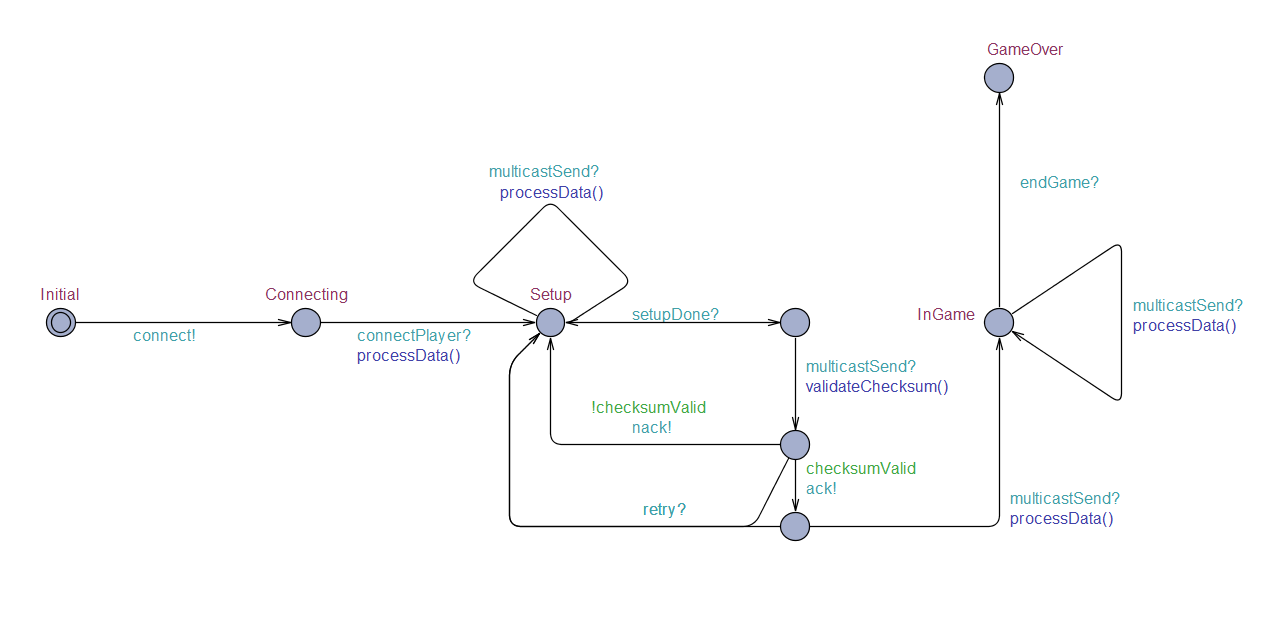
\includegraphics[width=1\linewidth]{/uppaal/client1.png}
    \caption{First iteration of the \uppaal client template.}
    \label{fig:uppaal-client-1}
\end{figure}

\begin{figure}[H]
    \centering
    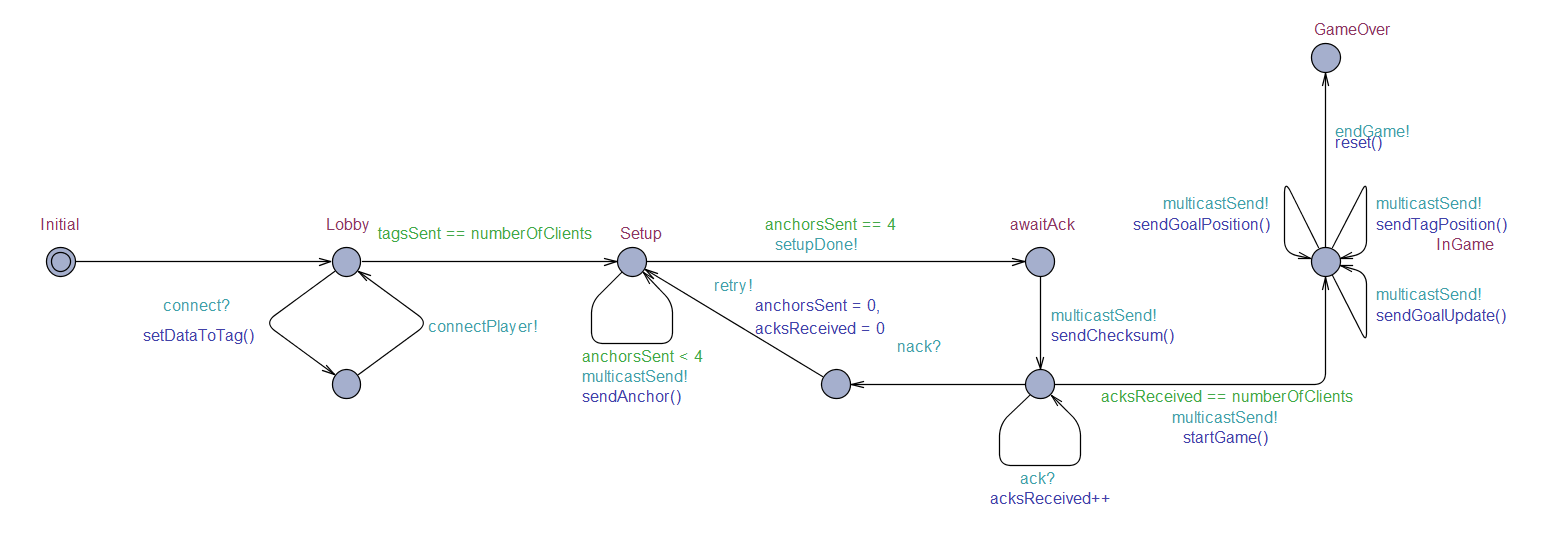
\includegraphics[width=1\linewidth]{/uppaal/host1.png}
    \caption{First iteration of the \uppaal host template.}
    \label{fig:uppaal-host-1}
\end{figure}

\subsection{Walkthrough of the model}
The model for the client is fairly straight forward, it starts in an \uppLoc{initial} location which indicates that the client is not yet trying to connect to the host.
The connection happens on the edge from the initial location to the \uppLoc{connecting} location.
In the model, this is represented with the client utilizing the channel \uppChan{connect}, and waiting for the host to synchronize by listening to the same channel.
When the synchronization happens, the host will execute the \uppFunc{setDataToTag()} function, which updates the data it is transmitting, and uses the channel \uppChan{connectPlayer} to inform the client that connection is now ready.
The client will call a function \uppFunc{processData()} to read the content of the buffer and react accordingly.
These steps will happen until the amount of \uppVar{tagsSent} is equal to the number of clients specified in the configuration.

\subsubsection{Setup}
The next location for both the host and client is \uppLoc{Setup}, which is the point where the host will transmit the anchor positions and ensure that all clients have consistent data.
The host will attempt to send the anchors one at a time with the \uppFunc{sendAnchor()} function until it has sent all 4 anchors to the clients.
Unlike the \uppChan{connect} and \uppChan{connectPlayer} channels, this happens on a broadcast channel, which allows multiple clients to receive the data at once to simulate the use of multicasting.
Since there is a chance that not all clients have received the four anchor coordinates correctly, the host will broadcast a checksum and have the clients either acknowledge or negative-acknowledge that the checksum is equal to the checksum of the data they have received.
In case any client returns a negative-acknowledge (using the channel \uppChan{nack}), all clients will go back to the setup and receive the anchor coordinates again until all clients send acknowledgements.

\subsubsection{InGame}
Finally, both the client and host will go to the \uppLoc{InGame} location to imply that the game is now happening.
To simulate asynchronous tasks, the host will continuously take a non-deterministic choice between sending a goal position, a tag position, a goal update or ending the game.
Meanwhile, the client only has two choices: Process data received on the multicast or wait for the game to end.

\subsubsection{Code aspect}
Behind the model, there are a series of variables and functions to make it all work.
In the global declarations the number of clients is specified, as well as an integer array called data, which is used as a buffer to transmit data between the host and clients, to simulate the internet connection in the real implementation.
The array has space for 5 elements to conform to the data format specified in \autoref{subsec:data-format}, such that the first element in the array will always be the type, which allows the client to act based on that when \uppFunc{processData()} is called.
The concrete implementation of \uppFunc{processData()} can be seen on \autoref{lst:uppaal:processData}.
For this iteration of the \uppaal model, updating player and goal positions are not implemented, since it did not seem like a significant detail to the model.

\begin{uppaalcode}[caption={Processing Data in \uppaal model}, captionpos=b,label={lst:uppaal:processData}]
void processData(){
    int type = data[0];
    
    if(type == 0){
        int anchorId = data[1];
        anchorsX[anchorId] = data[2];
        anchorsY[anchorId] = data[3];
        anchorsReceived++;
    } else if(type == 1){
        // Player position
    } else if(type == 2){
        // Goal position
    } else if(type == 3){
        // Score update
    } else if(type == 4){
        // Tag received
        tag = data[1];
        playerId = data[2];
    } else if(type == 5){
        // Setup checksum
    } else if(type == 6){
        // Start game
    }
}
\end{uppaalcode}
\noindent
Likewise, when the host has to send data, it will update the first element of the buffer and fill in the relevant data in the other elements.

\subsubsection{Checksum}
A checksum will be calculated on the client for checking whether or not the client has the correct setup information, and based on the checksum that the host broadcasts, the players will return either an acknowledge or negative-acknowledge.
\\
This checksum is simply calculated as the sum of all four anchor coordinates, as seen in \autoref{lst:uppaal:checksum}.

\begin{uppaalcode}[caption={Calculating checksum in \uppaal model}, captionpos=b,label={lst:uppaal:checksum}]
    void sendChecksum(){
        int checksum = 0;
        int i;
        for(i = 0; i < 4; i++){
            checksum += anchorsX[i];
            checksum += anchorsY[i];
        }
        data[0] = 5;
        data[1] = checksum;
    }
\end{uppaalcode}

\subsection{Updates to the network protocol}\label{subsec:sprint3networkupdate}
A good side-effect of generating the \uppaal model was that it required some reflection upon the network data format specified in \autoref{subsec:data-format}.
This resulted in some minor refactoring of the format.
\\
First of all, the format for sending a field anchor position had a timestamp as a part of the package.
Since the anchors will only be sent once, it does not make sense to timestamp it so this has been removed.
The updated version of the data format can be found in \autoref{app:network}.
\\
\autoref{tab:goal-zone} has been updated to be 8 bit and not 16 bit.
With 8 bit for the goal zone offsets, goals can not be larger than 255 cm x 255 cm, but we decided that it is a reasonable size.
Alternatively, the size could be increased to 16 bit, resulting in the goal zones having a maximum size of 655.36 m x 655.36 m, which would give the user room for customization to have much larger goal zones, but we deemed goal zones larger than 255 cm x 255 cm unnecessary for the time being.
Additionally, three new packages have been specified: Sending a player tag, sending an acknowledgement or sending the signal to start the game.

\begin{table}[H]
    \centering
    \begin{tabular}{|l|l|l|l|l|}
        \hline
        Offset (o) & POSY (y) & POSX (x) & TEAM\_ID (i) & \multicolumn{1}{c|}{\textbf{\begin{tabular}[c]{@{}c@{}}TYPE (t)\\ 5\end{tabular}}} \\ \hline
        8 bit      & 16 bit   & 16 bit   & 8 bit        & 8 bit                                                   \\ \hline
    \end{tabular}
    \caption{Format for goal zones.}
    \label{tab:goal-zone}
\end{table}
\begin{table}[h!]
    \centering
    \begin{tabular}{|l|l|l|}
        \hline
        \begin{tabular}[c]{@{}l@{}}PLAYER\_ID (p)\\ (1-4)\end{tabular} & \begin{tabular}[c]{@{}l@{}}TAG\_ID (i)\\ (0-65.535)\end{tabular} & TYPE (t) \\ \hline
        8 bits                    & 16 bits                   & 8 bits   \\ \hline
    \end{tabular}
    \caption{Format sending player tag.}
    \label{tab:player-tag}
\end{table}

\begin{table}[h!]
    \centering
    \begin{tabular}{|l|}
        \hline
        \begin{tabular}[c]{@{}l@{}}ACK (a)\\ (0-1)\end{tabular} \\ \hline
        8 bits                    \\ \hline
    \end{tabular}
    \caption{Acknowledge or negative-acknowledge.}
    \label{tab:acknowledge}
\end{table}

\begin{table}[h!]
    \centering
    \begin{tabular}{|l|}
        \hline
        \begin{tabular}[c]{@{}l@{}}TYPE (t)\\ 6\end{tabular} \\ \hline
        8 bits                    \\ \hline
    \end{tabular}
    \caption{Game start.}
    \label{tab:gamestart}
\end{table}
\noindent
The reason that \autoref{tab:acknowledge} does not have a type is that it is the only package that will be sent from the client to the host, so it will only need to contain a signal for the host to know whether the checksum is correct or not.

\section{Dead reckoning}
The accuracy of the representation of the players as well as the ball is important for the game to function well.
Since these positions are sent over the network, they might not always be the most recent positions, since they could be delay or packages lost.
\\\\
Dead reckoning is a technique that is used to predict where a game object is at current time based on its last know position, velocity and acceleration.
It is often used for networking games where packages about the object's kinematic state are continuously being sent from the server to the clients.
The kinematic state of an object includes its position, velocity, acceleration, orientation and angular velocity \autocite{DeadReckoning}.
If the client misses a package or they are not being sent often enough to have a new update for each frame, the representation of the object will jerk across the screen instead of having smooth and consistent movement.
That is where dead reckoning can be used to predict an objects movement to make it appear more believeable.
For the game we're building, it is important that each player's and the ball's positions are very accurate for the game to function properly.
\\\\
It is not possible have a new update for each frame, zero packet losses or zero latency. 
Therefore dead reckoning is needed to achieve a believeable representation of the ball and the players' movement \autocite{DeadReckoning}.
\begin{figure}[H]
    \centering
    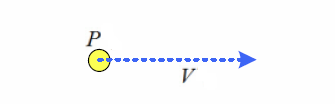
\includegraphics[width=0.6\linewidth]{dead_reckoning/dead_reckoning_example_1.PNG}
    \caption{Linear player movement}
    \label{fig:dead_reckoning_example_1}
\end{figure}
\autoref{fig:dead_reckoning_example_1} shows an example of a player's movement in the game.
In this example, dead reckoning would be a linear problem where the position, velocity and acceleration can be used to predict where the player will move to in the future. 
The dead reckoned position for a specific time $Q_t$ in this example can be calculated by:
\begin{displaymath}
    Q_t = P'_0 + V'_0T + \frac{1}{2}A'_0T^2
\end{displaymath}
where $ P'_0 $ is the position, $ V'_0 $ is the velocity, $ A'_0 $ is the acceleration and $T$ is the time \autocite{DeadReckoning}.
\begin{figure}[H]
    \centering
    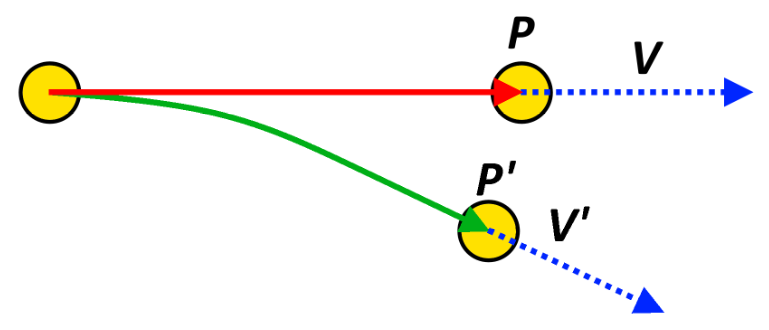
\includegraphics[width=0.6\linewidth]{dead_reckoning/dead_reckoning_example_2.PNG}
    \caption{A new update about the player's state is received from the server}
    \label{fig:dead_reckoning_example_2}
\end{figure}
In \autoref{fig:dead_reckoning_example_2} we receive a new update about the player's kinematic state. 
This results in conflicting realities when compared to the dead reckoned position calculated from the previous example. 
In the new update the player has turned right and a new dead reckoned position must be found, but this time it becomes a lot trickier since a believeable curve must be created from where we thought the player would be and where we estimate the player will be based on the new information. Representing the new position $P'_0$ immediately would result in the player warping across the screen which would not be ideal. Instead the player is represented at $ P_0 $ where we thought the player would be and the player should then move towards a new dead reckoned position, calculated with the information from the new update \autocite{DeadReckoning}.


\subsection{Projective Velocity Blending}
To calculate the curve that the player's movement needs to follow we need a good algorithm that is not too CPU intensive.
The algorithm must work well for a segment of a curve that is passing through two points being the player's current position $P_0$ and the estimated future location $P'_1$.
The recommened approach for this problem is projective velocity blending \autocite{DeadReckoning}.
\\\\
We create projections for the current kinematic state and the last known kinematic state and then these are blended together. 
\begin{displaymath}
    P_t = P_0 + V_0T_t + \frac{1}{2}A'_0T_t^2 \quad \rlap{\text{(Projecting from where player was)}}
\end{displaymath}
\begin{displaymath}
    P'_t = P'_0 + V'_0T_t + \frac{1}{2}A'_0T_t^2 \quad \rlap{\text{(Projecting from last known)}}
\end{displaymath}
\begin{displaymath}
    Q_t = P_t + (P'_t - P_t)\hat{T} \qquad \rlap{\text{(Combination of the two)}}
\end{displaymath}
\\\\
From this we get the dead reckoned location $ Q_t $ at the specified time. 
The reason that $ A'_0 $ is used in both projections is that it will converge to the player's true path much faster and it reduces oscillation, compared to when using $ A_0 $ when calculating $ P_t $. 
However, these calculations will still give inadequate results since the player's movement will have bad oscillations. 
These are cause by the changes in velocity,$V_0$ and $V'_0$, when new updates are received from the server. To account for this, a linear interpolation between the old velocity and the last known velocity is computed, which creates a blended velocity $V_b$. 
This velocity is used in the projection from where the player was, when a new update is received. 
This is what is known as \textit{projective velocity blending} \autocite{DeadReckoning}.
\\\\
\begin{displaymath}
    V_b = V_0 + (V'_0 - V_0)\hat{T} \quad \rlap{\text{(Velocity blending)}}
\end{displaymath}
\begin{displaymath}
    P_t = P_0 + V_bT_t + \frac{1}{2}A'_0T_t^2 \quad \rlap{\text{(Projecting from where player was)}}
\end{displaymath}
\begin{displaymath}
    P'_t = P'_0 + V'_0T_t + \frac{1}{2}A'_0T_t^2 \quad \rlap{\text{(Projecting from last known)}}
\end{displaymath}
\begin{displaymath}
    Q_t = P_t + (P'_t - P_t)\hat{T} \qquad \rlap{\text{(Combination of the two)}}
\end{displaymath}
This should reduce the oscillations in the player's movement significantly.
\begin{figure}[H]
    \centering
    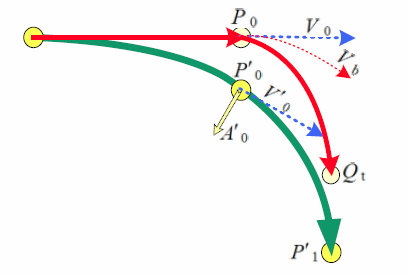
\includegraphics[width=0.6\linewidth]{dead_reckoning/dead_reckoning_example_3.PNG}
    \caption{Shows the the curve for the dead reckoned position $Q_t$ when making use of projective velocity blending}
    \label{fig:dead_reckoning_example_3}
\end{figure}
In \autoref{fig:dead_reckoning_example_3} we see the red curve that the player should follow to reach the dead reckoned position $Q_t$. $ P_0 $ is where we currently represent the player. $ P'_0 $ is the recent position received from the server. The green curve is the one that the player actually follows.
\\\\
This technique would be ideal to implement in the game if we find that the representation of the players' movement is inconsistent and in need of improvement.
\section{Sliding window protocol}
In \autoref{subsec:data-format} it was decided that the format of timestamps would be an integer from 0-255, where 0 to 20 would be considered as newer timestamps than 235 to 255.
However, if all the timestamps between 0 to 20, there would not be any updates until it has looped to a number between 0 and 20 and sent new updates.
To find a better solution to sliding window protocol was researched.
\\\\
Sliding window protocols are often used where reliable data is required.
Whenever the senders has sent the window sized packets, it waits for acknowledgement from the receiver before it sends new packets.

Each packet gets a sequence number and the acknowledgement sends back this number.
By doing this the receiver can keep track of the packets, and know which order is the correct one.
It can also discard duplicates and identify which packets are missing.
\\\\
As seen on \autoref{fig:sliding-window} an illustration of the sliding window has been made.
The sender will send the packets until the sliding window is full.
The sender will then wait for an acknowledgement from the first send packet in the window before it will send a new packets.

\begin{figure}[H]
    \centering
    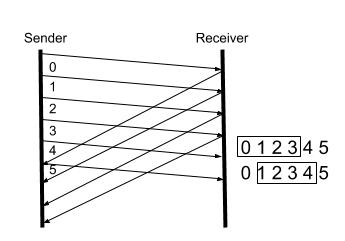
\includegraphics[width=0.6\linewidth]{sliding-window-illustration.jpg}
    \caption{An illustration of sliding window, where the window size is 4.}
    \label{fig:sliding-window}
\end{figure}
\noindent
For our project reliable data in the format of goal zones and goal score is important, however the player position is not important that it is reliable.
This is due to prioritizing that the update rate is higher and hereby we previously choose to use UDP in \autoref{subsubsec:choosing-between-udp-or-tcp}.
With Sliding Window protocol a player position would be retransmitted if it previously failed, and failed positions are quickly becoming outdated.
TCP already uses sliding window for flow control \cite{ibm:sliding-window}.

\section{Sprint 3 conclusion}\label{sec:sprint3conclusion}
This section concludes the preceding chapter on sprint 3.
It will recapitulate the knowledge that was obtained based on the sections of the chapter, and discuss the retrospective meeting that was held in the end of the sprint.

\subsection{Current product}
To give an overview of the progression of the project this section will provide an overview of what has been created during the sprint.
This overview will be split into two categories to reflect the structure of the project: Networking and game.

\subsubsection{Networking}
The major focus for the network part this sprint was to generate an initial UPPAAL model to visualize the flow of data.
This initial model is based on the assumption that packages are not lost and timeouts will not happen for simplicity.
Creation of this model lead to some revision to the network protocol as described in \autoref{subsec:sprint3networkupdate}.\\
In addition to the UPPAAL model, the ideas behind dead reckoning were examined in relation to this project.
The technique was deemed relevant to implement if the representation of the players' movement is inconsistent, which will be delved further into when the game is connected with the actual Pozyx location data.

\subsubsection{Game}
The most major changes in terms of the game this sprint was the addition of goal zones.
The goal zones were previously generated on the client, but to ensure a consistent game state across all clients, this has been moved to the host and will be transmitted over the network instead.
This meant that the major focus for the game in this sprint was refactoring how goals were displayed, as described in \autoref{subsec:goalrefactoring}.

\begin{figure}[H]
	\centering
	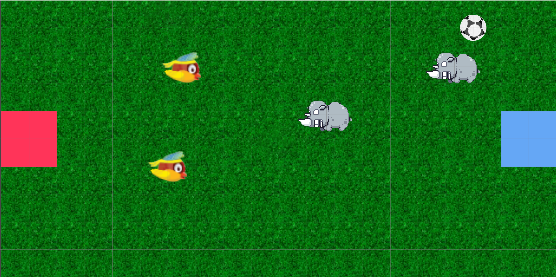
\includegraphics[width=0.6\linewidth]{sprint3/gamestatus.png}
	\caption{The current game status with goals and textures. This is a work in progress photo taken in Unity. The green rectangle is the playing field, and the smaller squares on either side are the goal fields. The birds and rhinos represent players, and the ball represents the ball being used for play. The white camera in the center is a Unity representation of where the camera is placed.}
	\label{fig:sprint3status}
\end{figure}
\noindent
Additionally, some temporary textures have been added to the game to get rid of the pink playing field and square players.
These new textures can be seen on \autoref{fig:sprint3status}.

\subsection{Retrospective on the process}
The ideal outcome of this sprint was an MVP of the product, but unfortunately, this was not achieved due to various problems.
First of all, there was a series of problems with merge conflicts in auto-generated files in Unity, which lead to the agreement that only one pair of group members should work on Unity at a time to avoid unsolvable merge conflicts.
This lead to a major delay in the Unity development.\\
Additionally, due to the COVID-19 lockdown, we did not have an opportunity to test the system properly with external users to get their feedback on the current product, as well as what to focus on for the last two sprints.
In addition to discussing the progress of the process, the following points were brought up:

\subsubsection*{How does the process with Jira work?}
The process has generally been improved since the last retrospective, not having to spend time assigning priority points to every task is nice.
The challenger expressed that he would appreciate if more people contributed to the backlog suggestions since it can be difficult to continuously come up with new tasks.


\subsubsection*{How has pair programming been working?}
Implementing the pair programming practice has been good for productivity.
However, it has been hard to coordinate at times, since it requires two people to be free at the same time for a pair programming task to properly start.
In the future, a single person should start with the development and when someone is available to join at a later point they can do so.

\subsubsection*{How is the daily stand-up working?}
While the new format proposed in the last sprint's retrospective was effective for a few days, it was quickly forgotten.
To keep the stand-ups effective, the anchor should be better at enforcing the format to make sure that everyone knows who needs help, and what people are currently doing.

\subsubsection*{How are the reviews going?}
The pair review format for code does not seem to be working too well since it is usually procrastinated until the next morning because one of the two reviewers is busy with something else.
\\
The single-person reviews are also lacking at the moment, where people do not remember to check what they are assigned to.
It is suggested that people regularly go to the front page of GitHub and check the "Recent Activity" which shows the pull requests you are assigned to.
It is also suggested that it is possible to ask people to review your code or text right away if it is important that it gets merged.
This is mostly if the task is blocking other tasks and thus is of great importance.


\subsubsection*{Closing comments}
Finally, we went through all the tasks that had been completed in the sprint to make sure that everything that was deemed important was described in the report.
It worked well, since it helped create an overview of the status of the project and figure out what to do next.


\chapter{Sprint 4}
\section{Updating the networking protocol}\label{sec:update-network-protocol}
During implementation of the networking protocol outlined in \autoref{sec:sprint3-uppaal}, problems related to the implementation of acknowledgements in the UDP based connection for game critical data were encountered.
Section \ref{sec:sprint3-uppaal} defines the way the protocol was envisioned to work based on the choice made in \autoref{sec:sprint1-networking}, where UDP sockets were selected as the type to be used for this project.
With the inherent unreliability of UDP due to the lack of reliable package delivery, and the importance of certain data being transmitted to players, it would be necessary to implement an acknowledgment from clients that they had received crucial data relating to the setup of the game, as defined in \autoref{sec:sprint3-uppaal}.
During the implementation of this, issues were encountered when sending the acknowledgment message from the client to the host.
As the sockets should make use of multicasting, as defined in \autoref{sec:sprint1-udptransmission}, our theory was that the clients should just be able to send messages to the same multicast group, and have the host receive that message, with a type that specified that the message was an acknowledgment that could be either positive or negative, structured in the same way as described in \autoref{subsec:data-format}.
However, the host had issues receiving the messages, where the message would be sent to the multicast IP, but never received by the host.
This prompted a discussion regarding how to remedy this issue, as a new approach seemed necessary.
Three main alternatives were considered:
\begin{itemize}
    \item Split the networking into two distinct phases - setup and in-game data
    \item Expand the messages being sent to include the crucial data on all messages sent
    \item Introduce a TCP element to make use of its reliability for game critical data
\end{itemize}

\subsubsection{Splitting networking into two distinct phases}
This approach aims to create a clear delineation between the crucial data that requires acknowledgment from clients and the data for which acknowledgments are unnecessary.
This was roughly the original approach, as shown on \autoref{fig:uppaal-host-1}, which illustrates how the host would wait in a setup state until acknowledgments had been received from all clients, and then the game would start.
This presents issues in terms of the multicast grouping, in which the host was unable to read messages sent through the group.
This could be remedied by having a separate multicast group in which clients could send acknowledgments, to avoid further problems related to multicasting.
While the host was sending out the information, a client could check if it had received the correct information, and if not send out a negative acknowledgment before timing out, to attempt to receive the information again.
Eventually all the clients would be sending positive acknowledgments.
\\\\
However, a limitation exists with this approach: when scoring a goal, it is crucial that the goalzones are moved.
This change of goal position would take place during the in-game phase, and receiving the information about the location of the new goalzone is crucial, such that all payers know where to score.
As such, the phase split loses some of its purpose, as an acknowledgment would need to be sent from clients during the playing phase.

\subsubsection{Expanding messages}
In addition to the data defined in \autoref{app:network}, crucial data could be appended to all messages sent during play.
This would mean that whenever any message was received, it would include the required information, and no acknowledgment would be necessary as the clients normally will receive some messages if they are continuously sent.
This would have the detriment of increasing the size of each individual package.
While the packages are currently not large enough to where this is likely to cause a problem, creating minimal packages is still a worthwhile goal in order to increase the speed of transmission and decoding.

\subsubsection{Introducing TCP}
On top of the currently described UDP approach to sending messages to ensure recent data is used for positioning while the game is played, a TCP socket connection between the host and clients could be implemented.
As described in \autoref{sec:sprint1-networking}, TCP includes reliability.
This reliability ensures that every message sent will be received by the client, through built in acknowledgments and retransmissions.
This would remove the need for clients sending UDP acknowledgments for game crucial data, and also make the implementation of a sliding window as described in \autoref{sec:sliding-window} for UDP unnecessary.
Because of the reliability, and needing established connections, TCP messages could potentially be slower to transmit.
This would be the case if the TCP connection had to retransmit a message.
Retransmitting a message involves waiting for a timeout, which incurs the larger overhead in comparison to UDP. 
As one of the focuses for the project is creating a networking solution capable of continuously updating positional data at a rate that makes the in-game positioning feel like real time, this is not an ideal solution for transmitting the data when the game is being played.
\begin{table}[h!]
    \begin{tabular}{|l|l|l|l|}
        \hline
            & Plus                                                                                                            & Minus                                                                                                                         & Interesting                                                                                                                                                             \\ \hline
        TCP & \begin{tabular}[c]{@{}l@{}}Reliable\\ Built in acknowledgements\\ Two way communication\end{tabular}            & \begin{tabular}[c]{@{}l@{}}Slower than UDP\\ More overhead because\\  of reliability and\\ two way communication\end{tabular} & \begin{tabular}[c]{@{}l@{}}For critical messages that concern \\ the state of the game TCP ensures \\ that all players receive \\ the update.\end{tabular}      \\ \hline
        UDP & \begin{tabular}[c]{@{}l@{}}Faster than TCP\\ Less overhead because it is a \\ one way communication\end{tabular} & \begin{tabular}[c]{@{}l@{}}Not as reliable\\ No built in \\ acknowledgements\end{tabular}                                      & \begin{tabular}[c]{@{}l@{}}Because UDP does not ensure that \\ the clients have received the \\ correct packages it can send \\ updates faster than TCP.\end{tabular} \\ \hline
    \end{tabular}
    \caption{PMI analysis of TCP and UDP}
    \label{Tab:PMI-TCP-UDP}
\end{table}     
We performed a PMI (Plus Minus Interesting) analysis, as taught in the Software Innovation course, on both protocols to outline the strengths and weaknesses of TCP and UDP which can be seen in \autoref{Tab:PMI-TCP-UDP}.
As can be seen on the table, both approaches have specific use cases where they are useful and in our case we have use cases for both TCP and UDP.
As such, a combination is proposed - TCP for crucial data, and UDP for positional data.
The issue described above relating to goalzones can also be remedied through a combination.
Rather than send location for the new goalzones while the game was being played and waiting for an acknowledgment, this data could be sent on the TCP connection as well, to ensure it arrives.

\subsubsection{Final choice of updating}
Based on the three alternatives to remedy the issues encountered, introducing a separate TCP connection between the hosts and the clients to handle crucial data that requires acknowledgments seems like the ideal choice.
It avoids the confusion inherent in the unreliability of UDP requiring manual handling of acknowledgments, and avoids communication back and forth, while allowing fast update times for positional data through the UDP connection.
Facilitating these changes would entail a slight change in the deployment diagram shown in \autoref{fig:sprint2-deployment}.
An association would have to be added between the host and client nodes indicating the new TCP connection, which is shown on \autoref{fig:sprint4-deployment}.
The dependency between the host and client application has also been updated to indicate that the client depends on both configuration and positional data.
\begin{figure}[H]
    \centering
    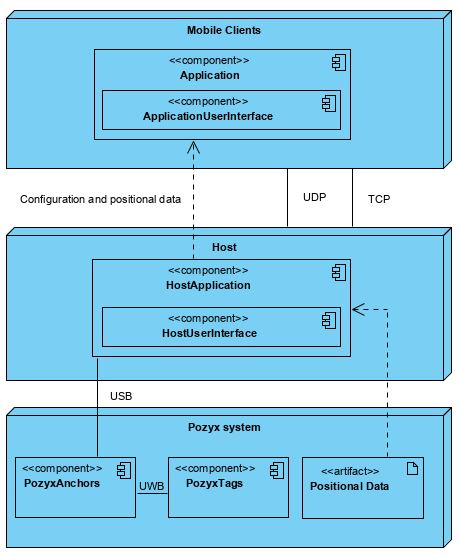
\includegraphics[width=0.6\linewidth]{sprint4/deployment-sprint4.JPG}
    \caption{A slightly revised deployment diagram for the system.}
    \label{fig:sprint4-deployment}
\end{figure}
\noindent

\section{Receiving information}\label{sec:receiving-the-information}
With the networking protocol in place, we will define how the data is received on the mobile clients.

The \texttt{in-game} scene in Unity has an \texttt{empty object} which handles receiving data from the UDP and TCP clients.
Having two separate clients allows them to run concurrently, so the UDP client does not block the TCP client or vice-versa.

\subsection*{UDP client}
Handling the datagrams on the UDP client is simple as it can currently only receive a packet with type 0 as defined in \autoref{app:network}, which is a packet containing a position for a Pozyx tag.

The datagram is received in the format \texttt{0xYYYYXXXXIISSTT} where 0x indicates hex and the rest of the identifiers are:
\begin{itemize}
    \item Y : Y position of the tag
    \item X : X position of the tag
    \item I : Id of player
    \item S : Timestamp
    \item T : Packet type
\end{itemize}

\noindent
When this datagram is received, we start by parsing the hexadecimal to a long datatype.
Since one hexadecimal corresponds to four bits we can get the type of the packet, which is the last two hex values of the datagram by typecasting it to a byte as seen on line 13 in \autoref{lst:readingudpdatagram}.

\begin{lstlisting}[caption={Processing datagrams in UDP client}, captionpos=b,language=C,label={lst:readingudpdatagram}]
private void DatagramHandler(string datagramMessage)
{
    // Remove 0x from string before parsing
    if(datagramMessage.ToLower().StartsWith("0x"))
    {
        datagramMessage = datagramMessage.Remove(0, 2);
    }

    long data;
    byte type;
    if (long.TryParse(datagramMessage, System.Globalization.NumberStyles.HexNumber, System.Globalization.CultureInfo.InvariantCulture, out data))
    {
        type = (byte)data;
        switch (type)
        {
            case 0:
                UpdatePlayerData(data);
                break;
            default:
                Debug.LogError("This type of message is not handled on UDP");
                break;
        }
    }
    else
    {
        Debug.LogError("Network data could not be parsed");
    }
}
\end{lstlisting}
\noindent
The next step in processing the data is calling the appropriate function as seen in the switch.
In this case we will take a look at the \texttt{UpdatePlayerData}, which is seen in \autoref{lst:updateplayerdata}.

\begin{lstlisting}[caption={Updating player data in UDP client}, captionpos=b,language=C,label={lst:updateplayerdata}]
private void UpdatePlayerData(long data)
{
    // bit shifting the hex value and typecasting to byte to get the values.
    // see network format in the report for more detail
    byte time = (byte)(data >> 8);
    byte id = (byte)(data >> 16);
    ushort x = (ushort)(data >> 24);
    ushort y = (ushort)(data >> 40);


    if (CheckTimestamp(time))
    {
        if (id == 0)
        {
            gameStateHandler.ballPosition.x = x;
            gameStateHandler.ballPosition.y = y;
        }
        else
        {
            // Player id starts at 1 while the playerposition array is 0 indexed. Decrementing id so that they line up.
            id--;
            gameStateHandler.playerPositions[id].x = x;
            gameStateHandler.playerPositions[id].y = y;
        }
    }
}
\end{lstlisting}
\noindent
The next step in processing the data is to read the actual content of the packet sent.
This is done by utilizing the fact that all parts of the packet have a size corresponding to a type in C\#.
The datagram is read from right to left using the right bit shift operation.
When a hexadecimal is bit shifted 4 bits to the right every decimal in the hexadecimal is moved one decimal to the right as illustrated on \autoref{fig:sprint4-bit-shift-basic}.

\begin{figure}[H]
    \centering
    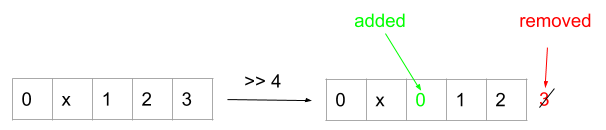
\includegraphics[width=0.6\linewidth]{sprint4/bitshift-illustration.png}
    \caption{Right bit shifting a hexadecimal by 4 bits.}
    \label{fig:sprint4-bit-shift-basic}
\end{figure}
\noindent
This can be utilized to read the different parts of the packet that the client received.
The first part that is read from the packet is the type of the packet.
In the packet the decimals representing the type are followed by two decimals representing the timestamp.
Because one digit corresponds to four bits, the packet has to be right bit shifted by 8 bits to move the timestamp to the back of the hexadecimal as illustrated on \autoref{fig:sprint4-bitshift-timestamp}.
\begin{figure}[H]
    \centering
    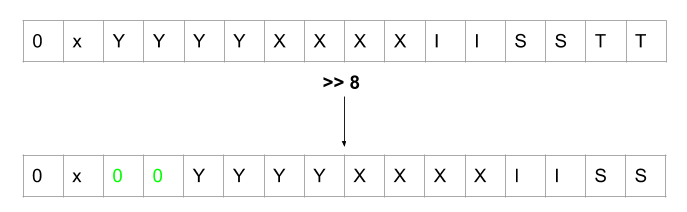
\includegraphics[width=0.6\linewidth]{sprint4/bitshift-timestamp-illustration.png}
    \caption{Bit shifting the packet to the right by 8 bits to get the timestamp to the back.}
    \label{fig:sprint4-bitshift-timestamp}
\end{figure}
\noindent
The packet can then be typecast to a \texttt{byte} to extract the timestamp from the packet.
The next part that is read from the packet is the player id.
Decimals representing the player id are followed by four decimals representing the x and y positions.
In order to get the player id to the back of the hexadecimal the packet has to be right bit shifted by 16 bits, illustrated on \autoref{fig:sprint4-bitshift-playerid}.
\begin{figure}[H]
    \centering
    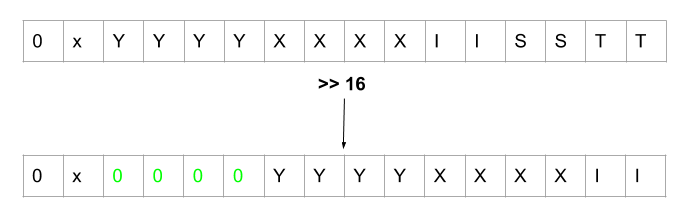
\includegraphics[width=0.6\linewidth]{sprint4/bitshift-playerid-illustration.png}
    \caption{Bit shifting the packet to the right by 16 bits to get the player id to the back.}
    \label{fig:sprint4-bitshift-playerid}
\end{figure}
\noindent
Because the player id is represented as two decimals it can be decoded from the packet by typecasting the packet to the \texttt{byte} datatype in C\#.
This is done for each part of the packet where the packet is bit shifted to the right by the combined size of the previously read parts and then typecast to a datatype that has the same size as the part of the message that is being read.
\subsection*{TCP client}
The principle behind the TCP client is much like the UDP client, where the type is read as a byte and then a switch statement ensures that the data is handled by the correct function.
However, since TCP is sent as a stream, all packets have been prefixed with numerical values to indicate the length of each packet.
This means that the client cannot simply wait for a new packet, read it and act according to the type.
Instead, the client will read the first two bytes of the stream and then read the incoming amount of bytes indicated by this numerical value, allowing the program to handle packet of varying length.


\chapter{Sprint 5}
\section{Sprint goal and introduction}
With the test results from the previous sprint, the main goal for this final sprint is first and foremost to correct the bugs that were discovered.
Since this is the last sprint, and it is a week shorter than the previous sprints due to time constraints, the focus is shifted from implementing major new features to polishing the currently existing features and prepare the system for a final test.
\section{Limiting the amount of UDP transmissions}
As the game was being tested we encountered a problem with the amount of UDP packages that were being transmitted.
Initially there were no limitations to the number of packages sent, and the server would transmit as many as it possibly could.
This would overburden the internet and could cause it to crash.
A limit had to be set for how many packages were able to be transmitted per second.
Since Pozyx can send updates on tags at a rate of approximately 60 per second, it would be preferable to have the limit at close to that amount.
The limit could even be a bit higher than 60, since the updates are being transmitted with UDP which means that there is no assurance that each package arrives.
Eventually, a limit of 70 packages per second was chosen based on the Pozyx limit and the chance of packages not arriving.
\\\\
\begin{lstlisting}[caption={Implementaion of the limit on the amount of packages that can be sent per second}, captionpos=b,language=C,label={lst:package_limitation}]
    self.time_now = time.time()
    if(self.time_prev != None):
        self.bytesAheadOfSchedule -= self.ConvertSecondsToBytes(self.time_now - self.time_prev)
    self.time_prev = self.time_now

    self.bytesAheadOfSchedule += 7
    if(self.bytesAheadOfSchedule > 0):
        time.sleep(self.ConvertBytesToSeconds(self.bytesAheadOfSchedule))

    # Send message to all clients listening on the multicast_group
    self.sendto(message, self.multicast_group)
\end{lstlisting}
The code from \autoref{lst:package_limitation} is from the send method of the UDP socket.
This code is run each time a UDP package is sent.
Initially the current time is stored, and the time difference between the current time and the time when the previous package was sent is converted to bytes.
The variable \texttt{bytesAheadOfSchedule} keeps track of whether or not too many bytes are being sent per second.
Since the size of the packages sent with UDP is always the same size, being 7 bytes, \texttt{bytesAheadOfSchedule} is incremented with 7 for each package sent.
If \texttt{bytesAheadOfSchedule} is above 0, too many packages are transmitted and the server should wait a bit before sending the next package using \texttt{time.sleep()}.
By doing this for each call to the \texttt{send} function, the number of packages sent per second can be limited to 70 per second.
\\\\
\begin{lstlisting}[caption={function for converting seconds to bytes and bytes to seconds}, captionpos=b,language=C,label={lst:conversion_functions}]
    def ConvertSecondsToBytes(self, numSeconds):
        return numSeconds*self.maxSendRateBytesPerSecond

    def ConvertBytesToSeconds(self, numBytes):
        return float(numBytes)/self.maxSendRateBytesPerSecond
\end{lstlisting}
\noindent
The conversion functions between bytes and seconds are seen in \autoref{lst:conversion_functions}.

\section{Evaluation on May 18th}\label{sec:evaluatin_test}
The evaluation of the system and all of its components took place on the 18th of May.
This was conducted as the previous test had not managed to explore the functionality of the game as described in \autoref{sec:initial-test}.
In the time between the two tests, the majority of the discovered bugs were fixed.
Due to the COVID-19 pandemic, the test was conducted using the group members as testers, and only one person from outside the group.
It would have been preferable to get external users to participate in the test, but this was obviously not a viable solution due to the circumstances.

\subsection{The setup}
The test was carried out in two phases, one inside and one outside.
The playing field was shaped like a rectangle for both tests, much like the previous test on the 7th of May as described in \autoref{sec:initial-test}.
An example of the setup can be seen on \autoref{fig:test2-indoor-setup}.

\subsection{Method and structure}
The test was largely unstructured, and was to an extent conducted as a big bang test.
Ideally, this test would have been conducted as a usability test, but as the group already had expert knowledge on how to operate the program, it is not possible to test the setup and the usability of the game.
Had a usability test been conducted, it would have been focused on the usage of the system as a player, meaning that a group member would have been in charge of setting up the Pozyx system and running the host computer.
The reason for this is that extensive knowledge about Pozyx is required to set up the game correctly, and that the host program has not been optimized for usability.
Neither of which are things that test subjects would be expected to be able to do.
Instead, they would have been given a short introduction about the game to see if they could understand and play the game, and the group would be present as observers.
Finally, at the end of the usability test, an interview would be conducted to get them to elaborate on their experience, with a special focus on how to make it more user friendly.
Further work into the preparation of a usability test has not been made, as it was deemed impossible to properly conduct the test due to the COVID-19 pandemic.

\subsection{Indoors test}
In the indoor test, the anchors were positioned as follows:
\begin{figure}[H]
    \centering
    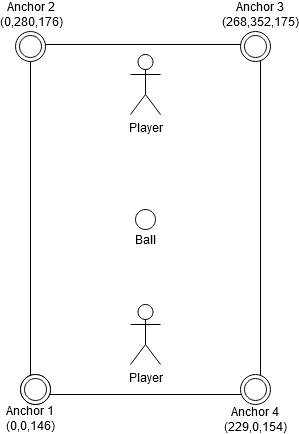
\includegraphics[width=0.5\linewidth]{usability/setupindoors.png}
    \caption{The setup for the indoors playing field. The coordinate at the anchors are in cm.}
    \label{fig:test2-indoor-setup}
\end{figure}
\noindent
During the indoor test it was discovered that two of the Pozyx tags did not correctly send positional updates even though they reported that everything was okay during the setup phase.
The tags would keep sending error codes that they could not identify themselves or that they could not find enough anchors to calculate their position.
As the two tags continuously kept reporting errors even when being run on a code example made by Pozyx themselves it was decided that it most likely was a hardware issue and would not be trivial to fix.
\\
The tests were instead successfully carried with one player on each team instead of the intended two players on each team.
The Pozyx positional updates arrived in a timely fashion, and the players were able to play against each other as intended with the remaining two player tags.
An issue in terms of playability was discovered, however.
If the playing field was suitably small, it was difficult for players to pass each other during play.
A picture of the gameplay in progress can be seen on \autoref{fig:usability-test-in-progress}.
\begin{figure}[H]
    \centering
    \includegraphics[width=0.5\linewidth]{usability/usabilitytestindoors.png}
    \caption{Test in progress indoors.}
    \label{fig:usability-test-in-progress}
\end{figure}
\noindent
They could simply just block each other, preventing goals from being scored.
Another point of interest was the inclusion of a physical ball in the design of the game, represented by a single Pozyx tag.
The reason a tag was used to represent the ball is that it seemed unlikely that the tag would be able to send positional data reliably and correctly enough if the tag were to be inserted into a ball since simply blocking the tag with a finger was enough to block any outgoing signals from it.
Additionally, inserting a tag into a ball and kicking it around could potentially damage the tag if it was not properly fastened securely in position.
Instead, the players were given their player tag and a small power bank to hold in their hands as seen on \autoref{fig:two-tags}, and the ball was attached to a larger power bank such that the players could easily distinguish the two tags even with a VR headset on.

\begin{figure}[H]
    \centering
    \begin{subfigure}{0.45\textwidth}
        \centering
        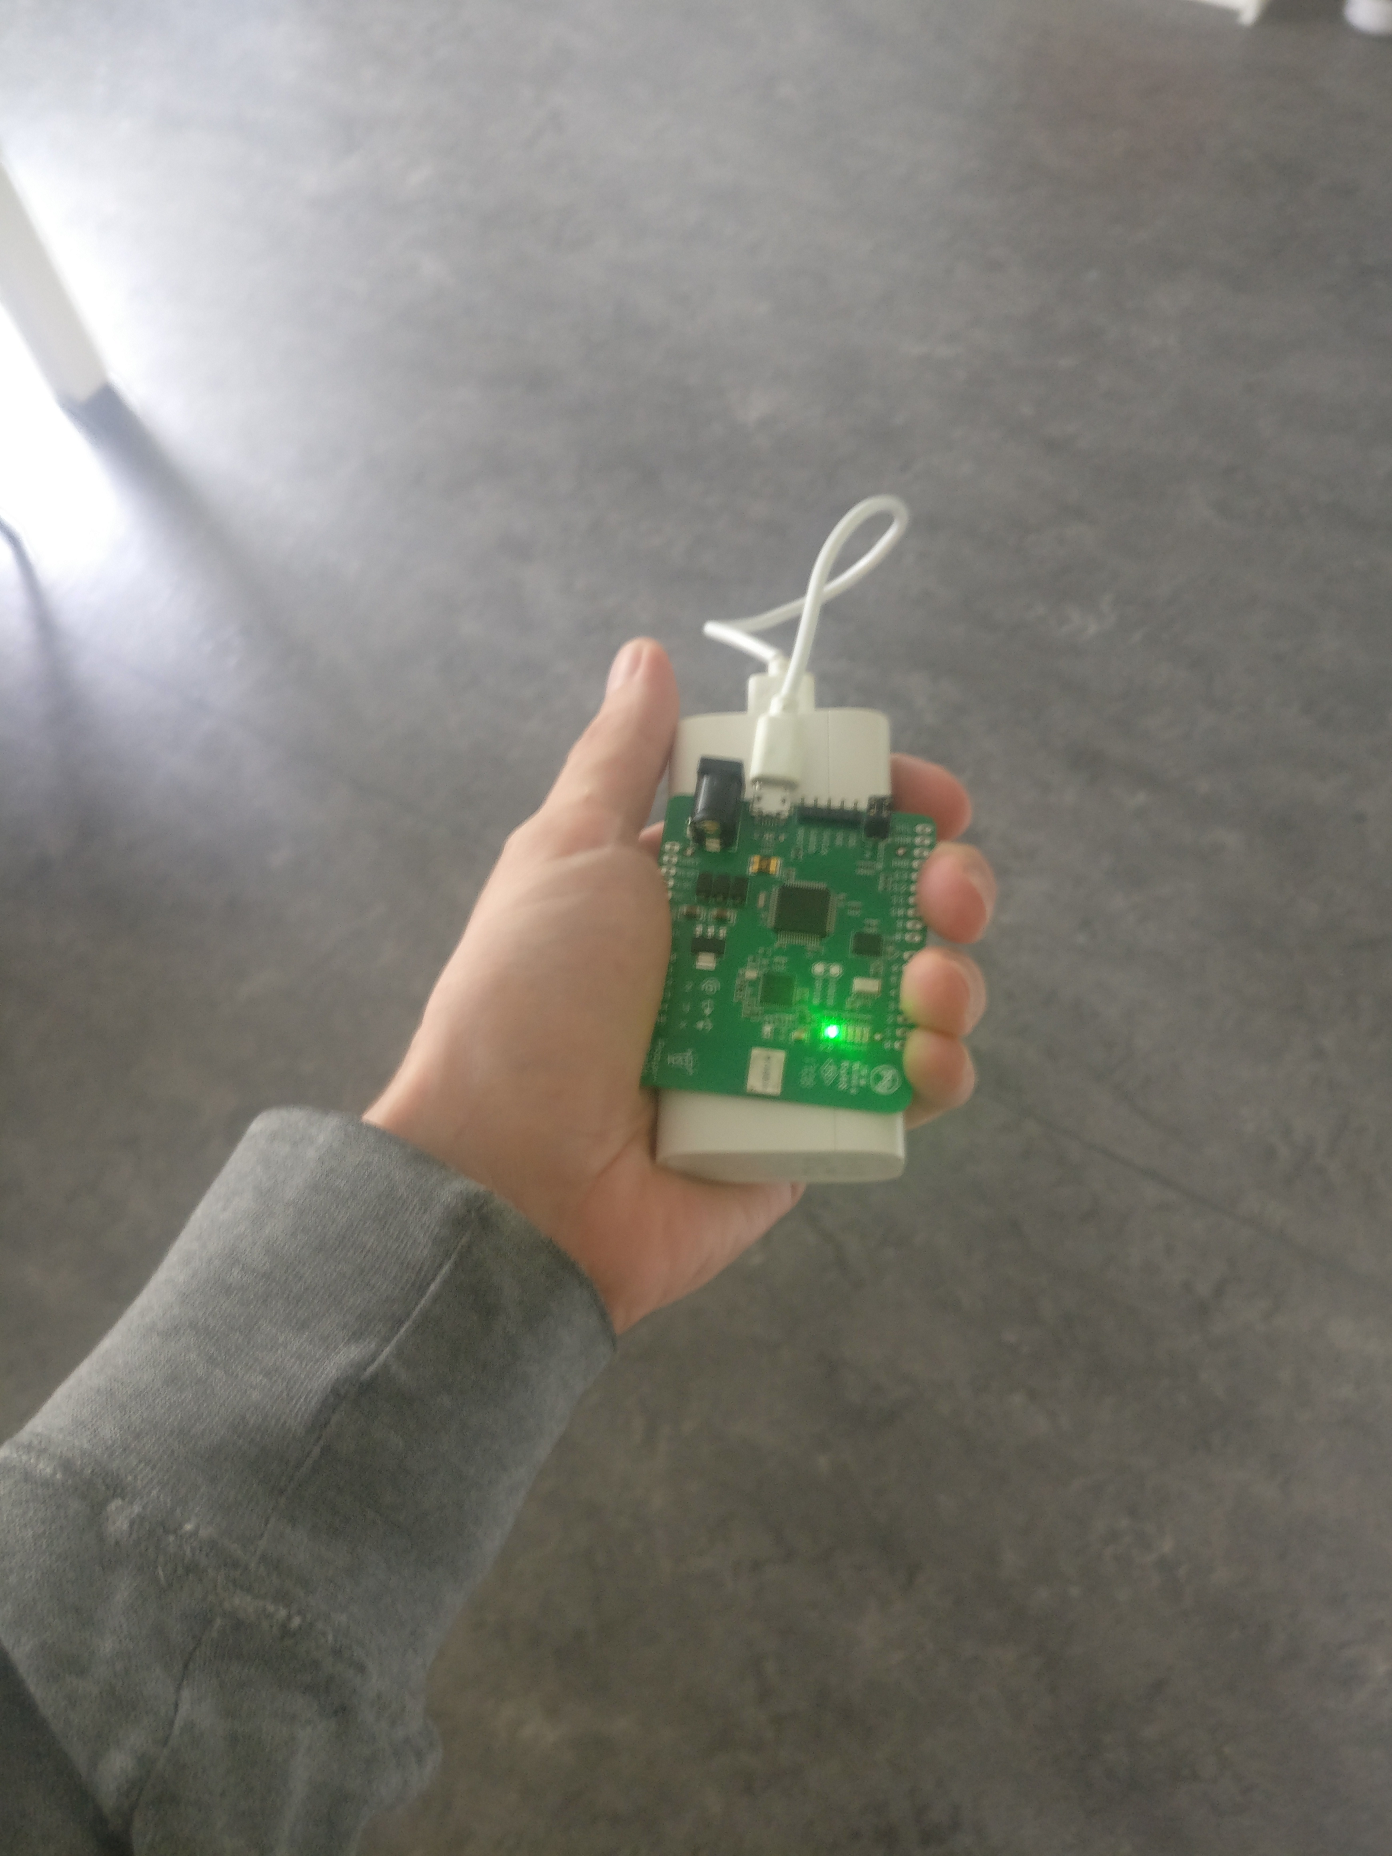
\includegraphics[width=0.8\linewidth]{usability/playertag.png}
        \caption{The player tag and a power bank.}
        \label{fig:sub1}
    \end{subfigure}
    \begin{subfigure}{0.45\textwidth}
        \centering
        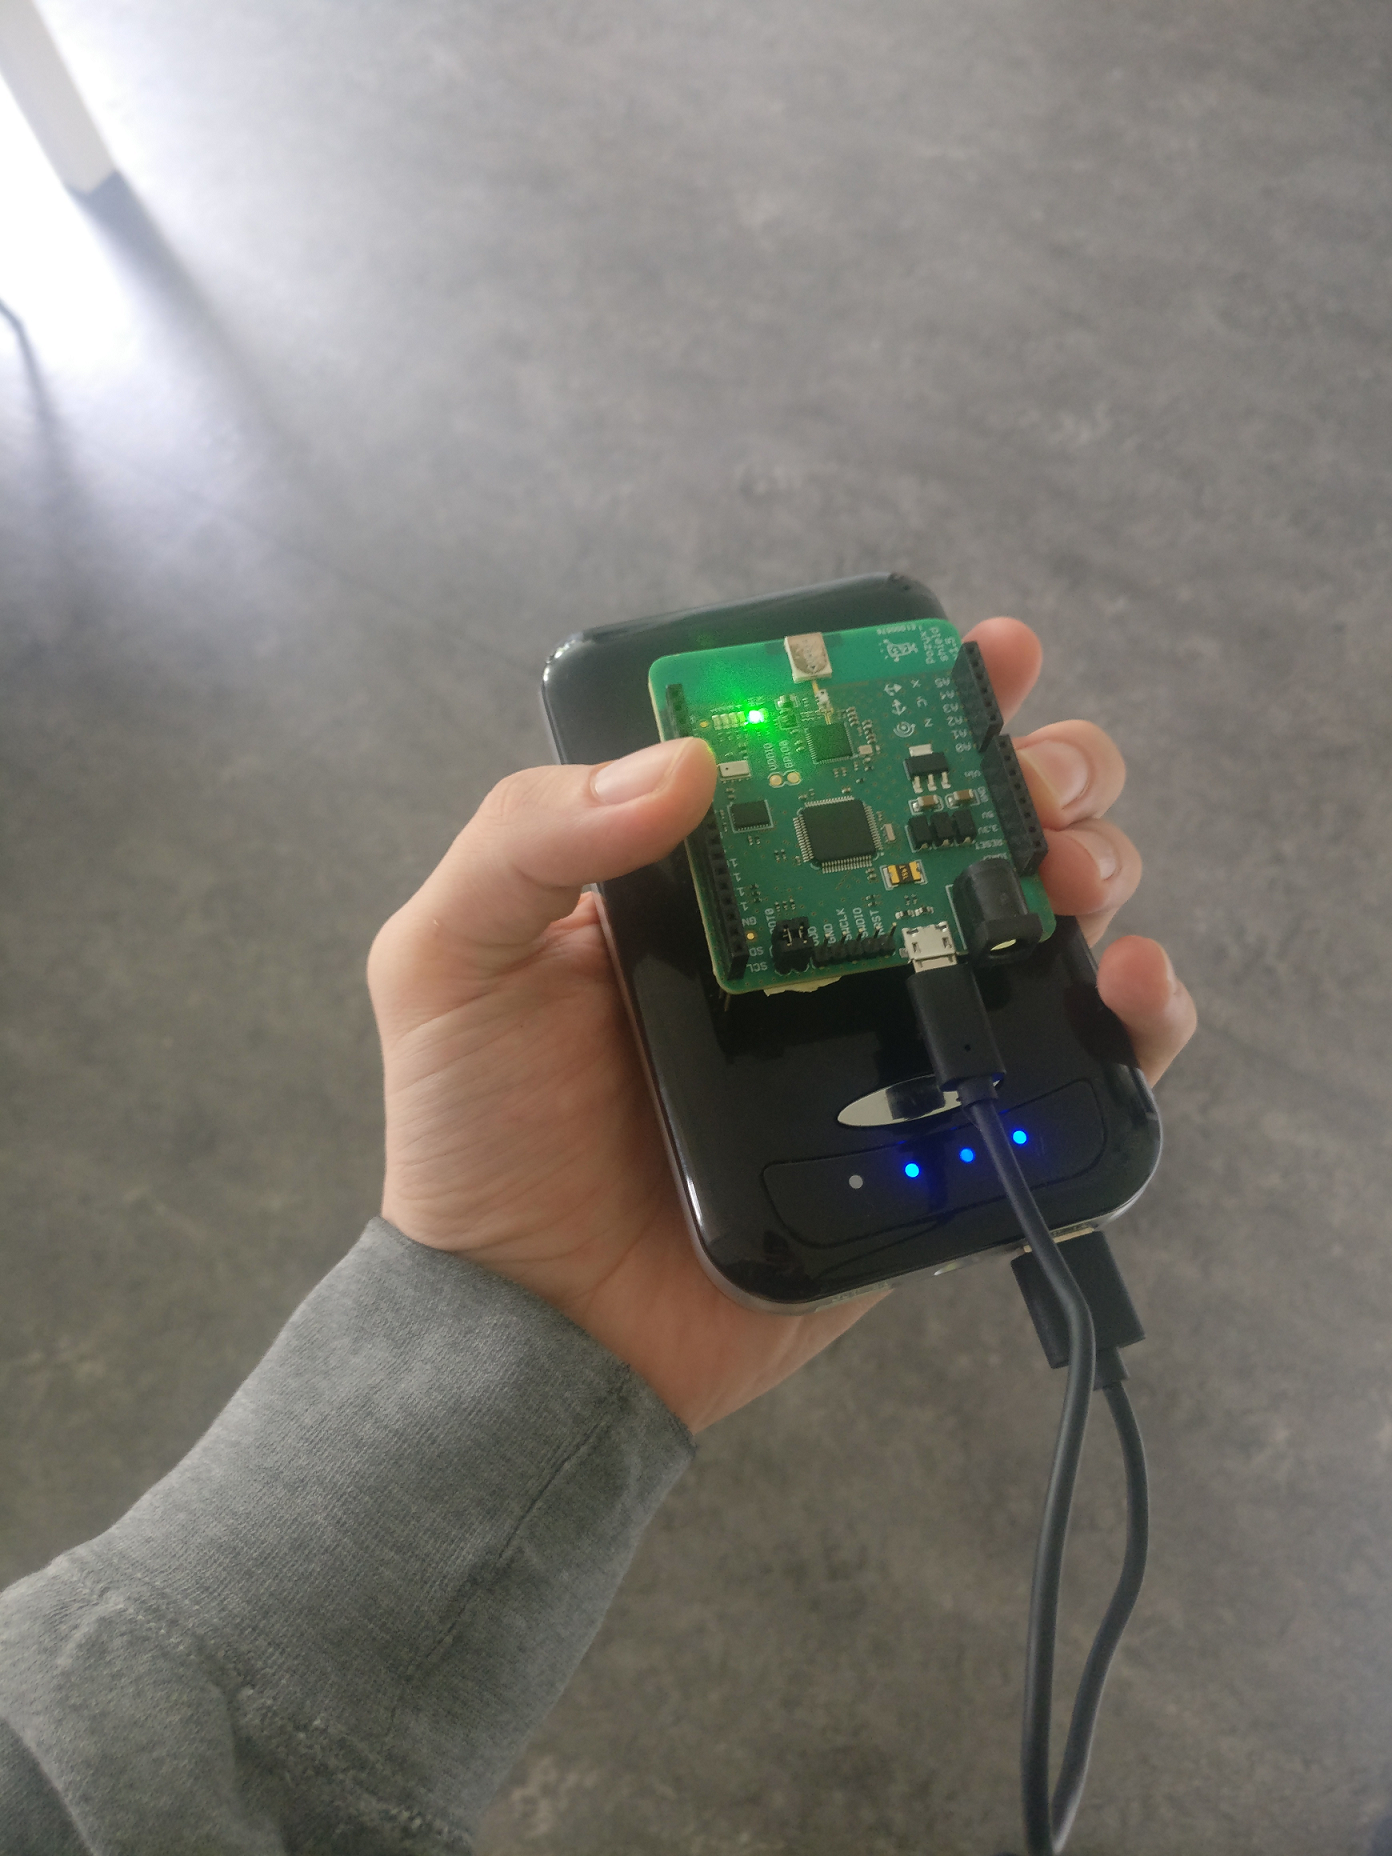
\includegraphics[width=0.8\linewidth]{usability/balltag.png}
        \caption{The ball tag and a power bank.}
        \label{fig:sub2}
    \end{subfigure}
    \caption{The tags used to show positions of players and the ball.}
    \label{fig:two-tags}
\end{figure}
\noindent
For the iteration of the game used for the test, there was no automatic transferal of the ball when players collided, and this is not possible with a physical ball.
As such, an extrinsic had to be implemented for further tests.
When colliding, the players would swap possession of the ball, and the player who previously had the ball would count down for a few seconds to allow the new player to gain some distance.
Once this rule had been implemented, the game could be played as intended.

\subsection{Outdoors test}
\begin{figure}[H]
    \centering
    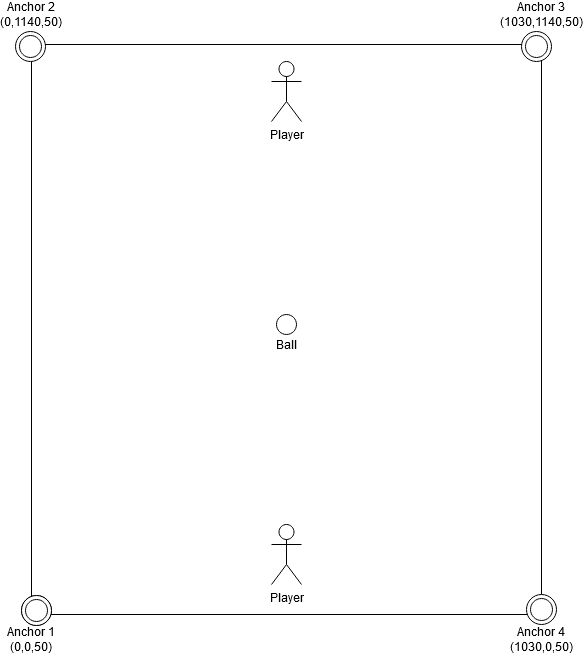
\includegraphics[width=0.5\linewidth]{usability/setupoutdoor.png}
    \caption{The setup for the outdoor playing field. The coordinate at the anchors are in cm.}
    \label{fig:test2-outdoor-setup}
\end{figure}
\noindent
In the outdoor test only three tags were used, the two player tags and the ball tag.
The setup for the outdoor test can be seen on \autoref{fig:test2-outdoor-setup}.
The field was constructed by placing the anchors on top of chairs placed in a rectangular shape, as can be seen on \autoref{fig:test2-anchor-setup}.
\begin{figure}[H]
    \centering
    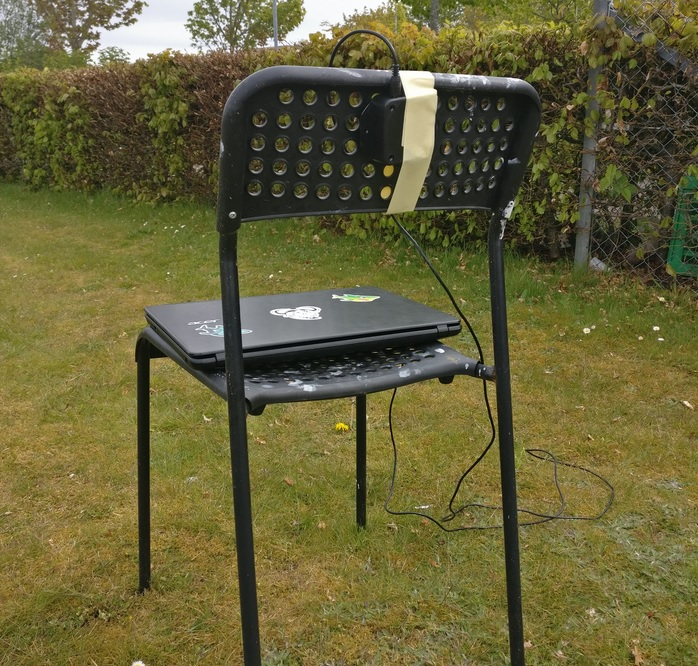
\includegraphics[width=0.4\linewidth]{usability/outdoor-setup.jpg}
    \caption{The setup of an anchor in the outdoor test.}
    \label{fig:test2-anchor-setup}
\end{figure}
\noindent
These anchors were connected to laptops or power banks to ensure no components would run out of power during play.
The game worked fine overall during the outside test, but the testers experienced that the tags sometimes stopped updating for several seconds.
Looking at the debug information available on the host laptop, it was easily seen that it periodically did not send any new positions to the clients, pointing towards a problem with the Pozyx hardware.
The updates of the players' positions would also not update as frequently some times and this could cause the movement of the players to appear quite janky, and resulted in less positional accuracy compared to the indoor test.
A picture of the gameplay outdoors can be seen on \autoref{fig:outdoor-gameplay}.
\begin{figure}[H]
    \centering
    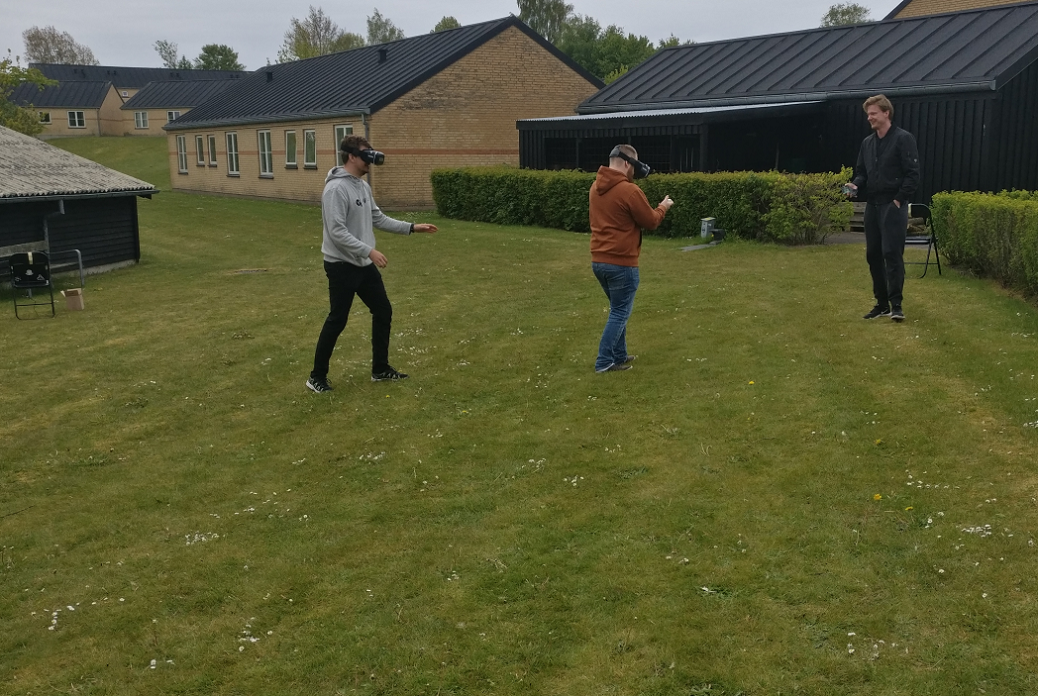
\includegraphics[width=0.6\linewidth]{usability/outdoorusabilitytest.png}
    \caption{Game in progress in the outdoors setup environment.}
    \label{fig:outdoor-gameplay}
\end{figure}

\subsection{Would this meet the users' requirements}
As we were unable to test on more than one person due to safety concerns related to COVID-19, it is limited how much information was gained from external users.
The external user did, however, have a few comments on the test:

\begin{itemize}
    \item It is impossible to see where you are positioned if you are outside the playing field.
    \item It is very unclear which goal is yours.
    \item It would be good if it was possible to see which direction you are turning.
    \item The update rate was quite slow in the outdoors test and the players are jumping from one position to another
\end{itemize}
Even though the game has a few lacking features, the user was entertained during the test of the game.

\subsubsection{Possible solutions}
There are two primary ways to solve the players not being able to see their position if they are outside the playing field.
The first would be the practical approach, where the field has a physical border to let the players know that they are at the edge.
Alternatively, it would be possible to add some padding around the in-game playing field, so the players can still see themselves until they are a given distance away from the field.
\\
To let the players know which goal is theirs, the player avatars could be colored according to their team color, or the goals could be colored according to their team's avatar.
\\
Letting the players see which direction they are facing could be solved by getting their tag orientation from Pozyx.
To ensure that the tag is always facing the same way as the user, the tag can be mounted on top of the VR headset as seen on \autoref{fig:tag-on-vr-headset}.

\begin{figure}[H]
    \centering
    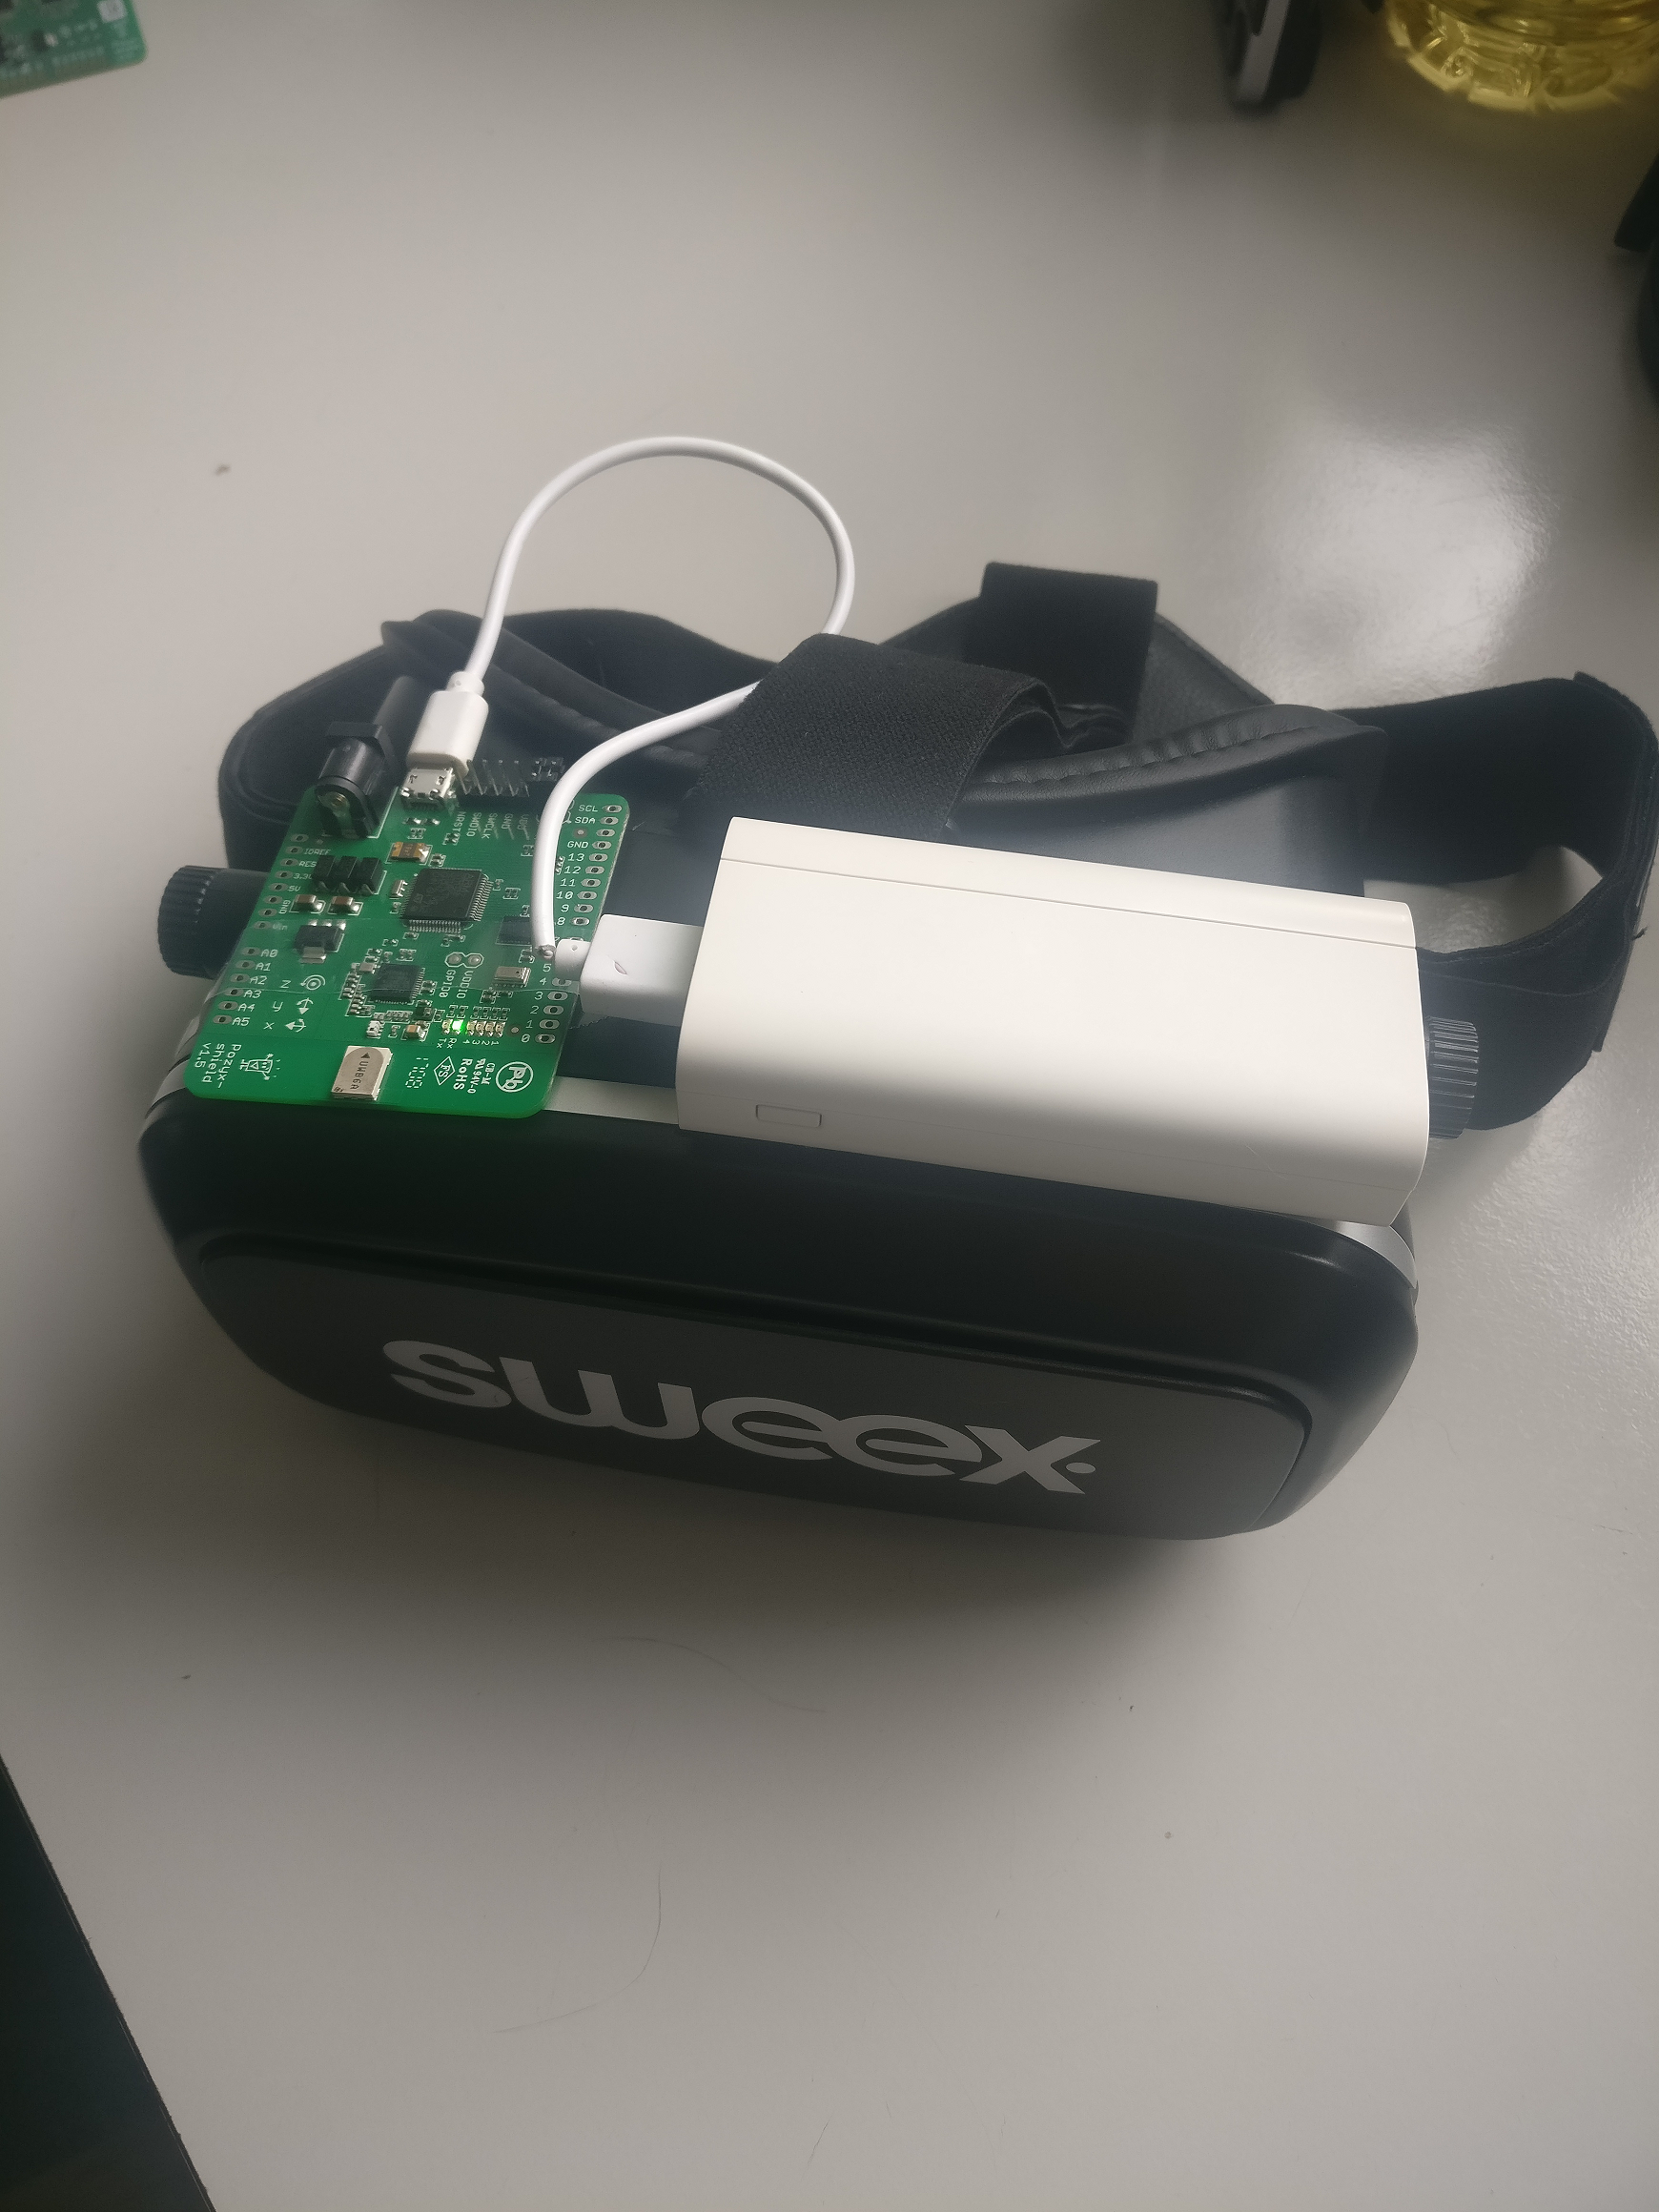
\includegraphics[width=0.4\linewidth]{usability/tagonvrheadset.png}
    \caption{Possible placement of Pozyx in future versions.}
    \label{fig:tag-on-vr-headset}
\end{figure}
\noindent
Finally, the problem with the update rate being slow is hard to fix, since it is a hardware limitation of Pozyx. However, it would be possible to implement dead reckoning to improve this.
To make the players move more smoothly from one position to another, linear interpolation can be used for rendering the move.

\section{Improving the movement of objects in the game}\label{sec:lerping}
The evaluation test of the game in \autoref{sec:evaluatin_test} revealed a problem connected to the slow update of the players' and the ball's positions.
The slow update rate made the movement of game objects jerky, meaning it was difficult for the players who were testing to have a real-time feeling of their position.
As discussed in \autoref{sec:dead-reckoning}, dead reckoning could be a possible solution to this kind of problem.
A requirement for dead reckoning is to have information about the acceleration and velocity of the different game objects.
Since the host was not able to provide this information to the clients, and due to time limitations, another solution had to be implemented.
Instead, the Unity function \texttt{lerping} was used, which finds the linear interpolation between two points.
By doing this, the movement of game objects can be animated between two positional points.
To achieve this the time when a new positional update is received needs to be stored for each of the game objects.
\begin{lstlisting}[caption={Calculating the position of the ball}, captionpos=b,language=C,label={lst:ball_position}]
    // Distance moved equals elapsed time times speed
    float totalTimeSinceLastUpdate = (float)(DateTime.UtcNow - gameStateHandler.timeAtLastUpdateBall).TotalSeconds;
    float distCoveredBall = totalTimeSinceLastUpdate  * gameStateHandler.ballSpeed;

    // Fraction of journey completed equals current distance divided by total distance.
    float fractionOfJourneyBall = distCoveredBall / gameStateHandler.journeyLengthBall;

    // Set our position as a fraction of the distance between the markers.
    var vector2CoordinatesBall = Vector2.Lerp(gameStateHandler.prevBallPosition, gameStateHandler.newBallPosition, fractionOfJourneyBall);
\end{lstlisting}
Lerping is calculated on the client-side and the code in \autoref{lst:ball_position} calculates the position of the ball for each frame.
For each frame, the time since the last update was received is calculated in seconds.
This value is multiplied with the speed of the ball to get the distance that the ball has covered between the last position and the new position.
Then the fraction of the journey is calculated by dividing the distance covered with the total journey length.
This value is then provided to the \texttt{Vector2.Lerp()} function as well as the old and new position which then calculates the current position of the ball.
The speed of the ball is dynamic in the way that it is calculated using the length between an old and new position and dividing that with the time it took between receiving the last two updates.
\\\\
Through testing with mock data, it shows that calculating linear interpolates for each frame results in a much smoother movement for each object in the game, which creates a more pleasant view for the players, as well as creating a more immersive and real-time feeling to the game.

\section{Final unity structure}
In unity there has been create two scenes: StartMenu, and Main scene.
This section will give an overview of these two scenes, and show the game objects that has been used in this project.

\subsection{Start menu}
The start menu is the lobby and the game objects within the scene can be seen on \autoref{fig:startmenu-game-objects}.
The five main game objects are the \texttt{GameStateHandler}, \texttt{ConnectionHandler}, \texttt{EventSystem}, \texttt{Menu}, and the standard \texttt{Main Camera}.
\\
The \texttt{GameState} contains a simple script with GameState information such as Anchor positions, player positions and other different variables used when the game start.
It also contains another script \texttt{DontDestroy}, which ensures that the game object does not get destroyed when changing scene.
\\
\texttt{ConnectionHandler} contains the scripts \texttt{DontDestroy} \texttt{TCPClient}.
The \texttt{TCPClient} receives the information from the host and adds the information received to the \texttt{GameState}.
\\
\texttt{Menu} has multiple gameobjects as children, which are used to specify how the UI should look.
The \texttt{ConnectButton} and \texttt{CancelConnection} uses an \texttt{OnClick} feature in unity, where it call as function to either connect or cancel the connection.
\\
The \texttt{EventSystem} supports sending events to objects based on input as clicks on button or typing in the text field.


\begin{figure}[H]
    \centering
    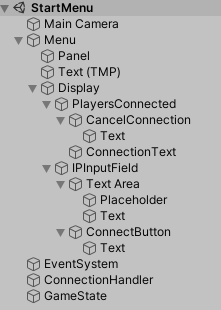
\includegraphics[width=0.4\linewidth]{figures/startmenu.PNG}
    \caption{The game objects in the start menu.}
    \label{fig:startmenu-game-objects}
\end{figure}

\subsection{Main scene}
The main scene is the game scene with the playing field.
The primary objects in main is \texttt{CLIENT}, \texttt{PlayingFieldContainer}, \texttt{Camera Rig} and \texttt{GvrEventSystem}.
These can be seen on \autoref{fig:main-game-objects}.
\\\\
The \texttt{CLIENT} contains the script \texttt{UDPClient}, which instantiates the UDP client and receives player and ball positions.
This script is previously described in \autoref{sec:receiving-the-information}.
\\
The \texttt{PlayingFieldContainer} only contains \texttt{PlayingField}.
The \texttt{PlayingField} has two children, where one of them is the GoalZoneController, which is used to generate the playing field and make sure that the entire field is visible with the camera.
The other is the \texttt{Goalscore-UI}, which is used to display the current score of the game.
It has two script attached to the gane object \texttt{FieldGenerator} and \texttt{PlayingFieldOffset}.
\texttt{FieldGenerator} creates the playing field from the coordinates coordinates in the \texttt{GameStateHandler}, which was instantiated in the lobby.
\texttt{PlayingFieldOffset} is used to change the center coordinate of the field, so that it has the same $x$ and $y$ position as the camera.



\begin{figure}[H]
    \centering
    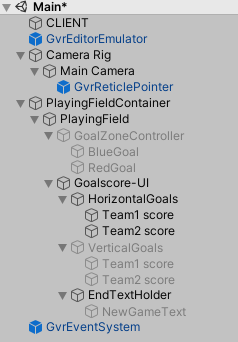
\includegraphics[width=0.4\linewidth]{figures/unity-main-gameobjects.PNG}
    \caption{The game objects in the main game scene.}
    \label{fig:main-game-objects}
\end{figure}


\section{Sprint 5 conclusion}\label{sec:sprint5-conclusion}
This section concludes the final sprint of this project.
Since it is the final sprint, no retrospective will be conducted with the aim to further improve the process.
In terms of the design and interface of the system, sprint 5 focused on testing the system to find potential issues, and fixing the bugs described in \autoref{sec:initial-test} and \autoref{sec:evaluatin_test}.
As such, the design was unchanged this sprint.
\section{Sprint 4 conclusion}\label{sec:sprint4conclusion}
This section concludes sprint 4 and will summarize the progress that has been made on the game and discuss the retrospective meeting conducted at the end of sprint 4.

\subsection{Current product}
The two current states of the game can be seen in \autoref{fig:sprint-4-state-of-game}.
We are currently able to connect to the host in the lobby, as seen on \autoref{fig:sprint-4-lobby}, which will lead to \autoref{fig:sprint-4-game} when the host has started the game.
\begin{figure}[H]
    \centering
    \begin{subfigure}{.5\textwidth}
        \centering
        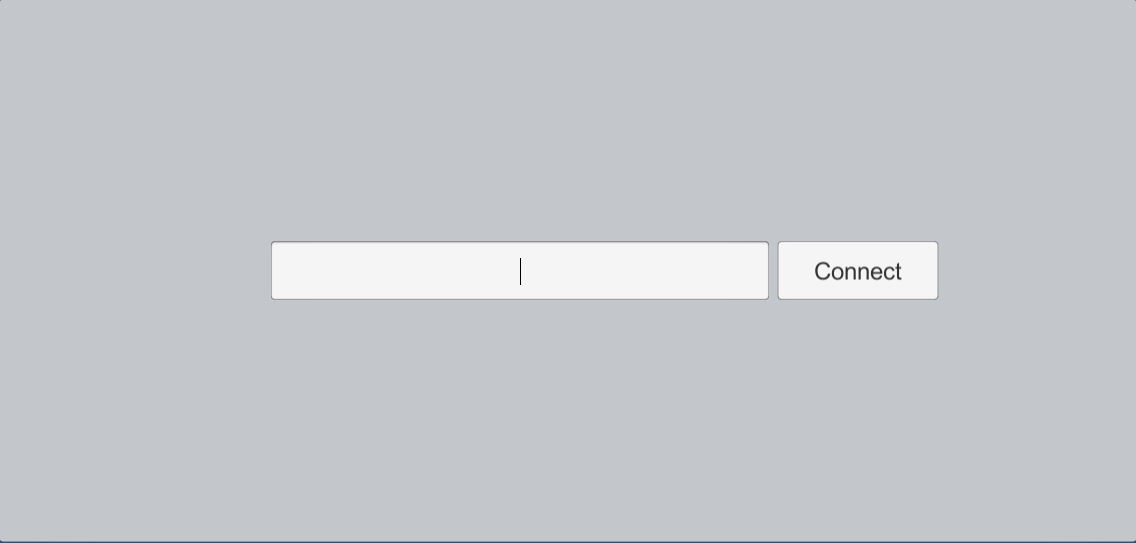
\includegraphics[width=1\linewidth]{figures/sprint-4-lobby.PNG}
        \caption{The lobby where you need to input the IP address to connect.}
        \label{fig:sprint-4-lobby}
    \end{subfigure}
    \begin{subfigure}{.4\textwidth}
        \centering
        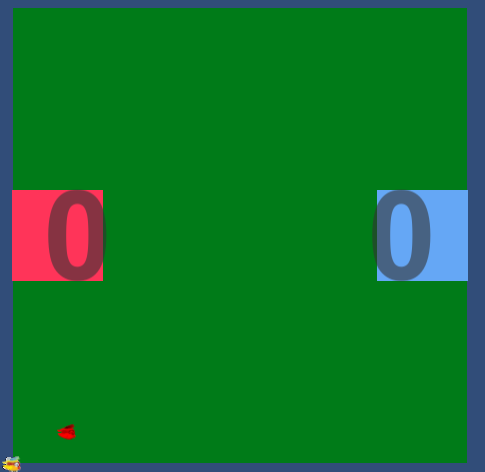
\includegraphics[width=.8\linewidth]{figures/sprint-4-game.PNG}
        \caption{The current playing field with goal zones, goal score and players.}
        \label{fig:sprint-4-game}
    \end{subfigure}
    \caption{The current state of the game}
    \label{fig:sprint-4-state-of-game}
\end{figure}

\subsubsection{Pozyx}
There are not many Pozyx programming tasks left, but there are some bugs that need to be fixed during the next sprint.
\\
During the initial test of the program described in \autoref{sec:initial-test} several exceptions occurred, which were caused by the input data not being correctly formatted.
This should be fixed in the following sprint.
Problems with the firmware were also discovered in the initial test, where Pozyx would not send positional data to the host, but only coordinates of $(0, 0, 0)$.

\subsubsection{Game}
If the problems with Pozyx get fixed, the game should have implemented the majority of the requirements defined for the MVP in \autoref{sec:mvp}.
However, in the current iteration of the game, the teams are unable to win the game.
This is a highly prioritized Unity task, which we intend to implement in the last sprint.

\subsubsection{Networking}
To be able to win the game, it is necessary for the host to be able to send a message that the game has ended to the clients.
Therefore a package needs to be specified for this purpose to be implemented along with the ability to win a game.
The host also needs to send information about the number of goals a team needs to score before they win the game, which requires the package containing player data to be updated to also include goal amount.

\subsection{Retrospective on the process}
This subsection will elaborate on the retrospective meeting that was held on May 12th.

\subsubsection*{How does the process with Jira work?}
The process with Jira will change with the last sprint.
For previous sprints there was a \textit{Suggested} column and a \textit{Discussed} column, but in the upcoming final sprint the \textit{Discussed} column will no longer be used.
Tasks will either be moved to \textit{Chosen for development} or a \textit{Future work} column that was added, rather than go through the \textit{Discussed} column.
The next sprint will be the last, and therefore it is necessary to prioritize it differently.
Either the task has to be completed, or it has to be documented in \textit{Future work}.

\subsubsection*{How has pair programming been working?}
Pair programming works well, but there are some challenges with online pair programming in Unity.
The main challenges are that, when testing, it is required that the game is compiled to an android device, which is more difficult to share with the other programmer unless they both compile the game.

\subsubsection*{How is the daily stand-up working?}
When the members of the group do not have a task, the daily stand up seems pointless, as they do not have much to say.
To change this, at the start of the day the developers should have five minutes to look at possible tasks for the day and pick one, so that they have the opportunity to discuss that during the stand-up meeting.
\\\\
There was also a comment that estimations of completed tasks were inaccurate.
Whenever someone estimated during a stand-up that they would have a task completed by the end of the day, it would often not be completed in time for the next stand-up.
The developer would then give the same estimation, saying it would now be done by the end of the day, and the pattern could repeat.
In order to remedy this, and attempt to ensure that the estimations could become more accurate, the developers should have to specify the reasons why they did not complete the tasks, if they exceeded the estimated duration of the tasks given in a stand-up meeting.
It is suspected that a possible cause of some of this lazy estimation could be that the motivation for certain tasks might be low, and to help this we will introduce pair report writing for larger report tasks, such that the developer pair can help keep each other accountable.

\subsubsection*{How are the reviews going?}
The group members are now more aware of doing the reviews after it was discussed in \autoref{sec:sprint3conclusion}, so reviews often get done at the same day or in the morning the next day.

\chapter{Appendix}


\printbibliography[heading=bibintoc]
\label{bib:mybiblio}
\listoffigures
\listoftables
\lstlistoflistings
\end{document}
